%%%%%%%%%%%%%%%%%%%%%%%%%%%%%%%%%%%%%%%%%
% Daily Laboratory Book
% LaTeX Template
%
% This template has been downloaded from:
% http://www.latextemplates.com
%
% Original author:
% Frank Kuster (http://www.ctan.org/tex-archive/macros/latex/contrib/labbook/)
%
% Important note:
% This template requires the labbook.cls file to be in the same directory as the
% .tex file. The labbook.cls file provides the necessary structure to create the
% lab book.
%
% The \lipsum[#] commands throughout this template generate dummy text
% to fill the template out. These commands should all be removed when 
% writing lab book content.
%
% HOW TO USE THIS TEMPLATE 
% Each day in the lab consists of three main things:
%
% 1. LABDAY: The first thing to put is the \labday{} command with a date in 
% curly brackets, this will make a new page and put the date in big letters 
% at the top.
%
% 2. EXPERIMENT: Next you need to specify what experiment(s) you are 
% working on with an \experiment{} command with the experiment shorthand 
% in the curly brackets. The experiment shorthand is defined in the 
% 'DEFINITION OF EXPERIMENTS' section below, this means you can 
% say \experiment{pcr} and the actual text written to the PDF will be what 
% you set the 'pcr' experiment to be. If the experiment is a one off, you can 
% just write it in the bracket without creating a shorthand. Note: if you don't 
% want to have an experiment, just leave this out and it won't be printed.
%
% 3. CONTENT: Following the experiment is the content, i.e. what progress 
% you made on the experiment that day.
%
%%%%%%%%%%%%%%%%%%%%%%%%%%%%%%%%%%%%%%%%%

%----------------------------------------------------------------------------------------
%	PACKAGES AND OTHER DOCUMENT CONFIGURATIONS
%----------------------------------------------------------------------------------------

\documentclass[hyperref,openany,10pt]{labbook} % 'openany' here removes the gap page between days, erase it to restore this gap; 'oneside' can also be added to remove the shift that odd pages have to the right for easier reading

\usepackage[ 
  backref=page,
  pdfpagelabels=true,
  plainpages=false,
  colorlinks=true,
  bookmarks=true,
  pdfview=FitB]{hyperref} % Required for the hyperlinks within the PDF

% Usual font and encoding package
\usepackage[utf8]{inputenc} % Required for the top and bottom rules in the table
\usepackage[T1]{fontenc} % Required for the top and bottom rules in the table
\usepackage[french]{babel} % Required for the top and bottom rules in the table

% For figures and tables
\usepackage{booktabs} % Required for the top and bottom rules in the table
\usepackage{float} % Required for specifying the exact location of a figure or table
\usepackage{graphicx} % Required for including images
\usepackage{subfigure} % Allow subfigure with their own caption

% Miscellaneous
\usepackage{lipsum} % Used for inserting dummy 'Lorem ipsum' text into the template
\usepackage{grffile} % changes the algorithm to check for known extensions (option multidot, enabled by default)

\usepackage{xcolor}
\definecolor{bl}{rgb}{0.0,0.2,0.6} 

\usepackage{sectsty}
\usepackage[title,titletoc,toc]{appendix}
\allsectionsfont{\color{bl}\scshape\selectfont}
\renewcommand{\sectfont}{\color{bl}\scshape\selectfont}

\usepackage[bottom=3.5cm]{geometry}

% For math
\usepackage{amsmath}

% For algorithms
\usepackage{algorithm,algorithmicx,algpseudocode}


\newcommand{\HRule}{\rule{\linewidth}{0.5mm}} % Command to make the lines in the title page
\setlength\parindent{0pt} % Removes all indentation from paragraphs
\setlength{\parskip}{\baselineskip} % add blanc space between paragraphs




%----------------------------------------------------------------------------------------
%	DEFINITION OF EXPERIMENTS
%----------------------------------------------------------------------------------------

\newexperiment{example}{This is an example experiment}
\newexperiment{example2}{This is another example experiment}
\newexperiment{example3}{This is yet another example experiment}
\newexperiment{table}{This shows a sample table}
%\newexperiment{shorthand}{Description of the experiment}

%---------------------------------------------------------------------------------------

\begin{document}

%----------------------------------------------------------------------------------------
%	TITLE PAGE
%----------------------------------------------------------------------------------------

\frontmatter % Use Roman numerals for page numbers
\title{
\begin{center}
\HRule \\[0.4cm]
{\Huge \bfseries Cahier d'expérience \\[0.5cm] \Large Master de Science des Données}\\[0.4cm] % Degree
\HRule \\[1.5cm]
\end{center}
}
\author{\Huge Victor Estrade \\ \\ \LARGE victor.estrade@u-psud.fr \\[2cm]} % Your name and email address
\date{Début $1^{er}$ Avril 2016} % Beginning date
\maketitle

\tableofcontents

\mainmatter % Use Arabic numerals for page numbers

%----------------------------------------------------------------------------------------
%	LAB BOOK CONTENTS
%----------------------------------------------------------------------------------------


\labday{Mardi, 5 avril 2016}

Expérimentation sur le correcteur. Je vais résumé ici mes résultats et remarques
sur l'utilisation d'un correcteur simple (une seule couche) pour apprendre par l'exemple
à inverser des transformations linéaires simples.

Pour ce j'utilise le modèle simpliste (figure \ref{fig:correcteur}). 
Sans utilisation d'adversarial.

\begin{figure}[H] % Example of including images
\centering
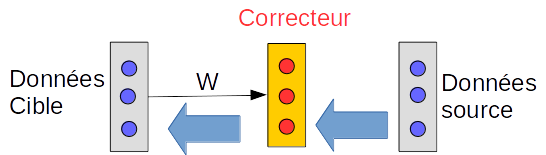
\includegraphics[width=0.45\linewidth]{fig/05-04-2016/Correcteur.png}
\caption{Correcteur simple}
\label{fig:correcteur}
\end{figure}

Le réseau est entraîné par minibatch avec un nombre d'époque prédéfini à la main.
La fonction de coût utilisée est la \emph{mean squared error} : $(x_{pred}-x_{vrai})^2$

Puisqu'il n'y a pas de \emph{décodeur} l'unique couche (unique matrice de poids $W$)
est constituée de $d$ neurone où $d$ est le nombre de descripteur des données.


\experiment{Corriger MNIST après transformations linéaires}

Dans un premier temps sur MNIST.
Le réseaux doit reconstruire l'image transformée.
MNIST est assez pratique car il permet de visualiser facilement l'efficacité 
de la reconstruction pour des données avec un bon nombre de descripteurs (748 pixels).

\subexperiment{Alignées}

Tout d'abord j'ai gardé la correspondance entre l'image original et
l'image transformée pendant l'entraînement du correcteur (cas aligné).
Ainsi chaque paire d'exemple $(x, \phi(x)) \in MNIST\times \phi(MNIST)$
contient uniquement l'information que l'on cherche $\phi$.

Ce qui donne de très bon résultats la plupart du temps.\\


{\Large\textbf{Mirror.}} On commence par une simple permutation des 
descripteurs de façon à renverser les images.

Le correcteur se débrouille sans souci, sans avoir besoin d'adversarial. Ceci
nous offre un exemple typique de cas où tout se passe bien. Les résultats sont résumés
figure \ref{fig:mnist_mirror_pairwise}.

\begin{figure}[H] % Example of including images
\centering
\subfigure[Sample images]
	{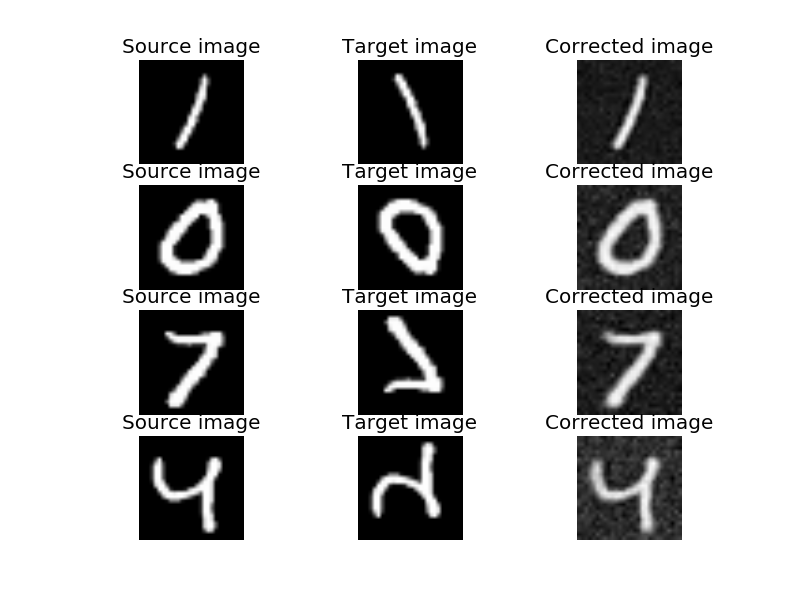
\includegraphics[width=0.45\linewidth]{fig/05-04-2016/MNISTMirror-PairWiseCorrector-lambda-0.0000-sample.png}}
\hfill
\subfigure[Learning curve (squared loss)]
	{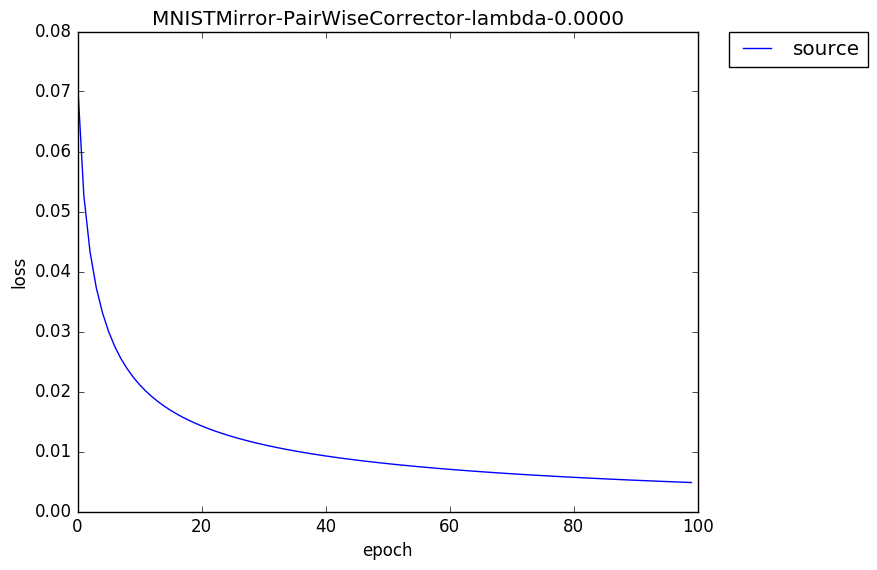
\includegraphics[width=0.45\linewidth]{fig/05-04-2016/MNISTMirror-PairWiseCorrector-lambda-0.0000.png}}
\subfigure[Weights]
	{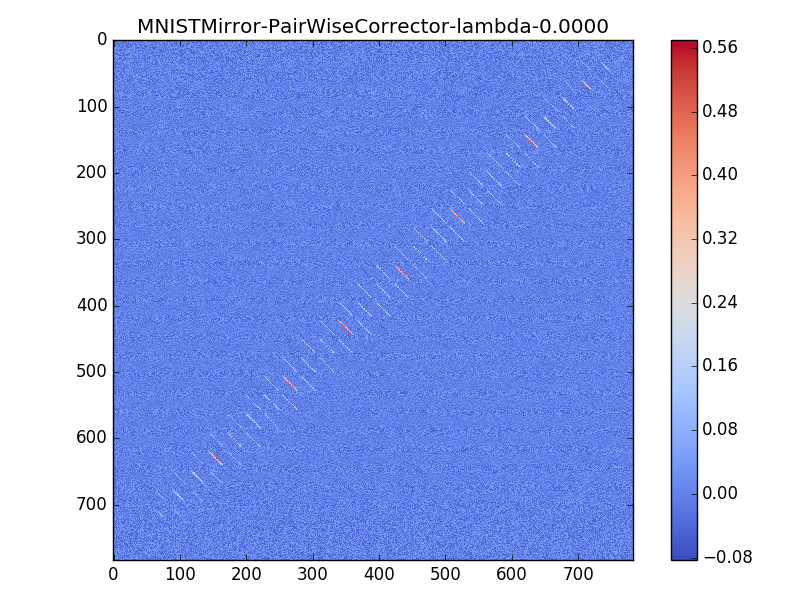
\includegraphics[width=0.45\linewidth]{fig/05-04-2016/MNISTMirror-PairWiseCorrector-lambda-0.0000-Weights.png}}
\caption{MNIST - Mirror correcteur aligné}
\label{fig:mnist_mirror_pairwise}
\end{figure}


{\Large\textbf{RMat.}} On se lance maintenant dans un problème légèrement plus
difficile pour la machine mais impossible pour l'œil humain, une transformation
linéaire aléatoire:
$$ \phi(x) = A.x$$
où $A$ est une matrice générée aléatoirement.

Pour éviter les problèmes d'échelle, les données ont été renormalisées après 
transformation (sinon : loss = NaN).

Les résultats sur cette transformation sont assez mitigés. De plus elle requiert
un entraînement particulièrement long (quelques centaines d'époques). Mais bon avec
les yeux de la fois et en choisissant les bons exemples ça a l'air de fonctionner.
Une fois de plus les résultats sont résumés figure \ref{fig:mnist_rmat_pairwise}.

\begin{figure}[H] % Example of including images
\centering
\subfigure[Sample images]
	{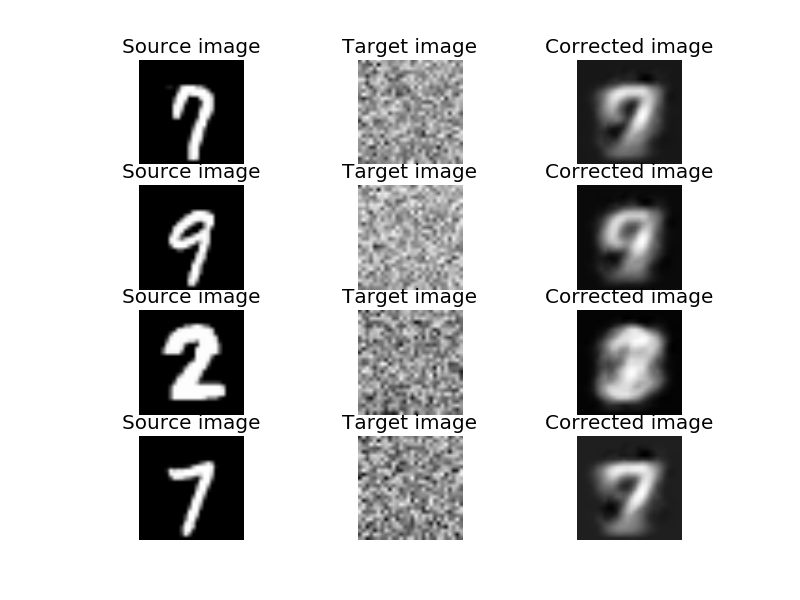
\includegraphics[width=0.45\linewidth]{fig/05-04-2016/MNISTRMat-PairWiseCorrector-lambda-0.0000-sample.png}}
\hfill
\subfigure[Learning curve (squared loss)]
	{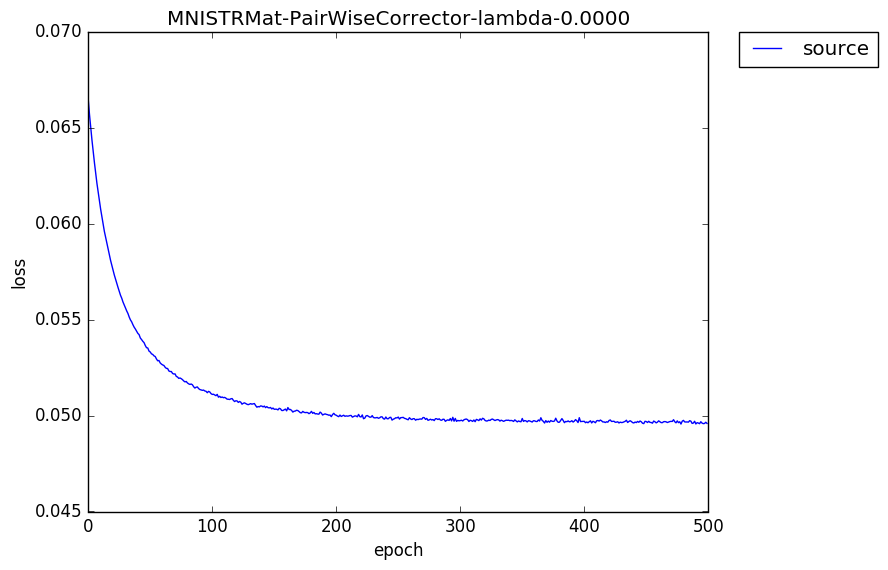
\includegraphics[width=0.45\linewidth]{fig/05-04-2016/MNISTRMat-PairWiseCorrector-lambda-0.0000.png}}
\subfigure[Weights]
	{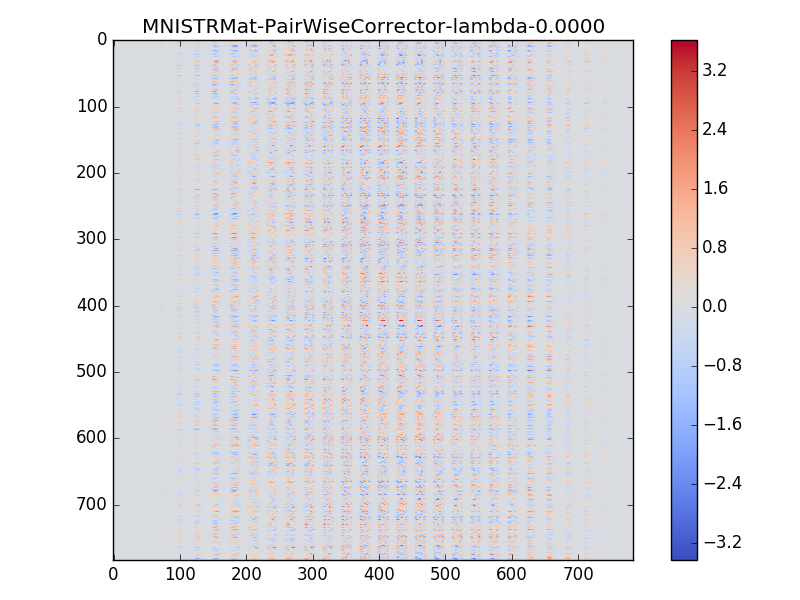
\includegraphics[width=0.45\linewidth]{fig/05-04-2016/MNISTRMat-PairWiseCorrector-lambda-0.0000-Weights.png}}
\caption{MNIST - RMat correcteur aligné}
\label{fig:mnist_rmat_pairwise}
\end{figure}


\subexperiment{Non alignées}

Ici chaque paire d'exemple $(x_i, \phi(x_j)) \in MNIST\times \phi(MNIST)$
ne contient pas uniquement l'information que l'on cherche $\phi$. Même si
les exemples $x_i$ et $x_j$ sont choisis parmi la même classe, ces exemples 
se différencient non seulement par la transformation subie mais aussi par 
les variations au sein d'une même classes.

Ceci est plus proche de cas d'expériences réels. Exemple: des échantillons
du même type sans être exactement les mêmes et utilisant des instruments
de précision différents.

L'entraînement est donc légèrement plus complexe. Pour le moment j'ai utilisé 
la version naïve où je sélectionne aléatoirement les exemples d'une même classe
pour être alignés. Cette sélection change à chaque nouvelle époque. Des 
améliorations possibles de cette technique seront développées plus loin.\\


{\Large\textbf{Mirror.}} à nouveau l'on commence par le cas simple des images 
miroirs. Cette fois ci la qualité des résultats est plus discutable. 

\begin{figure}[H] % Example of including images
\centering
\subfigure[Sample images]
	{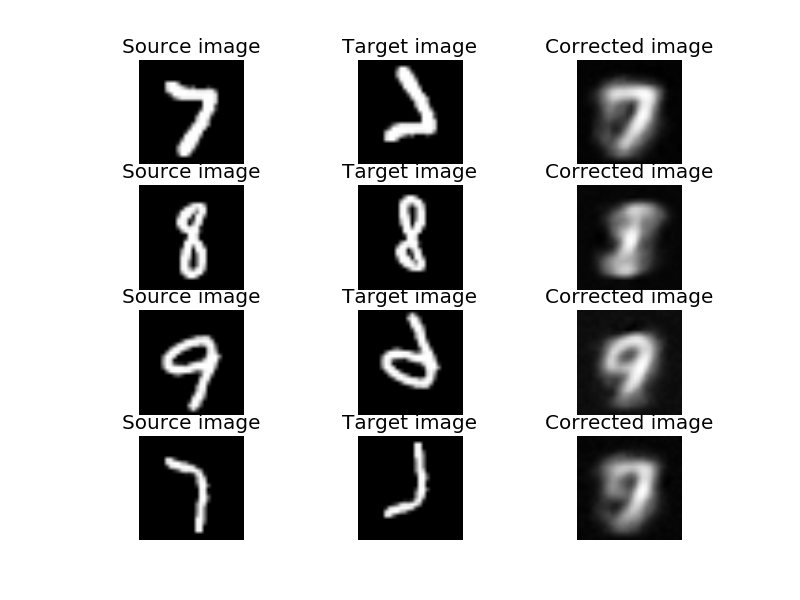
\includegraphics[width=0.45\linewidth]{fig/05-04-2016/MNISTMirror-ClassWiseCorrector-lambda-0.0000-sample.png}}
\hfill
\subfigure[Learning curve (squared loss)]
	{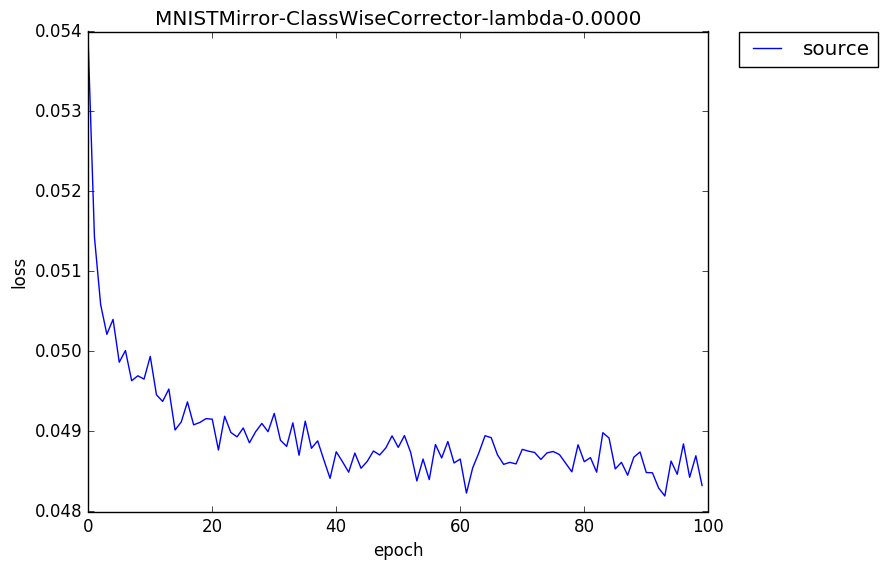
\includegraphics[width=0.45\linewidth]{fig/05-04-2016/MNISTMirror-ClassWiseCorrector-lambda-0.0000.png}}
\subfigure[Weights]
	{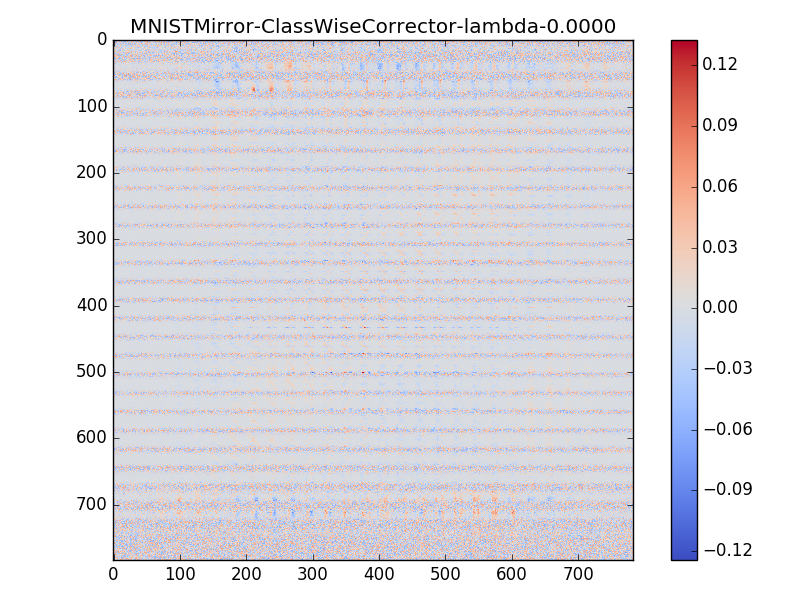
\includegraphics[width=0.45\linewidth]{fig/05-04-2016/MNISTMirror-ClassWiseCorrector-lambda-0.0000-Weights.png}}
\caption{MNIST - Mirror correcteur non aligné}
\label{fig:mnist_mirror_classwise}
\end{figure}


{\Large\textbf{RMat.}} On reprend la transformation linéaire aléatoire:
$$ \phi(x) = A.x$$
où $A$ est une matrice générée aléatoirement.


\begin{figure}[H] % Example of including images
\centering
\subfigure[Sample images]
	{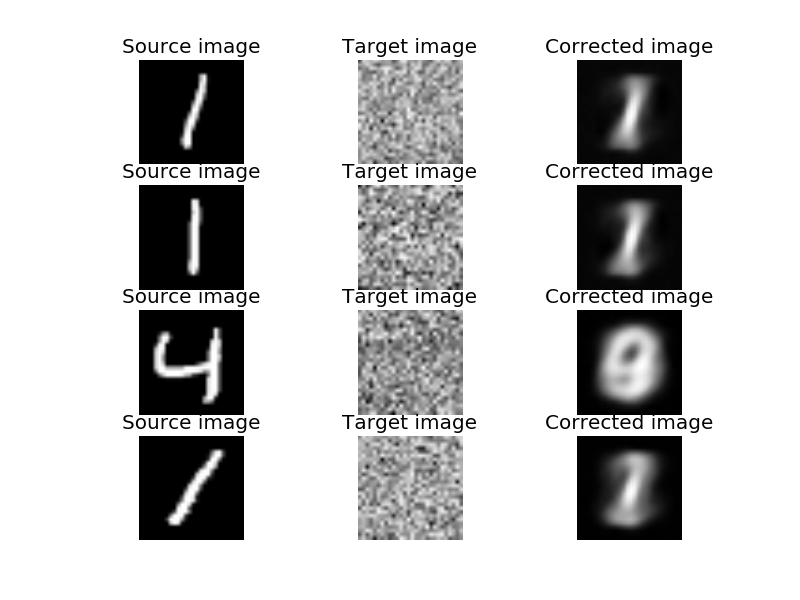
\includegraphics[width=0.45\linewidth]{fig/05-04-2016/MNISTRMat-ClassWiseCorrector-lambda-0.0000-sample.png}}
\hfill
\subfigure[Learning curve (squared loss)]
	{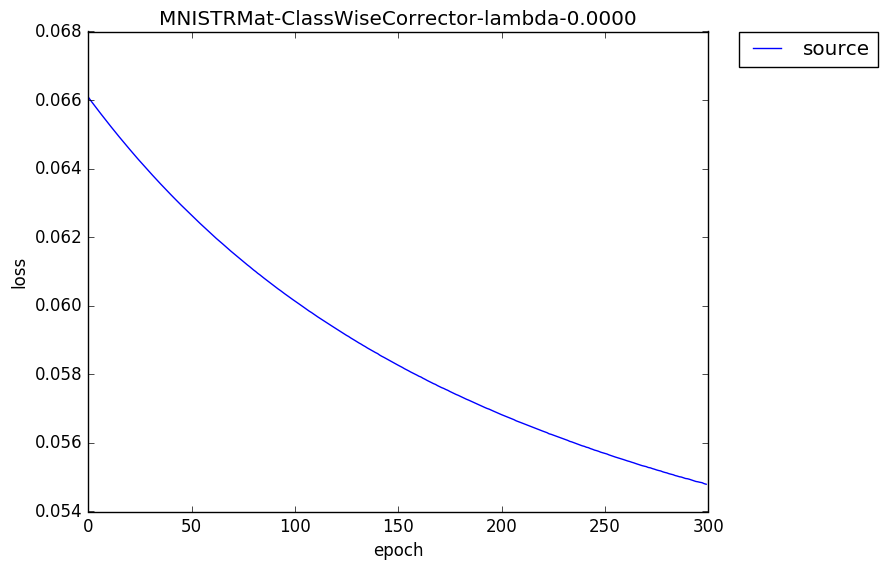
\includegraphics[width=0.45\linewidth]{fig/05-04-2016/MNISTRMat-ClassWiseCorrector-lambda-0.0000.png}}
\subfigure[Weights]
	{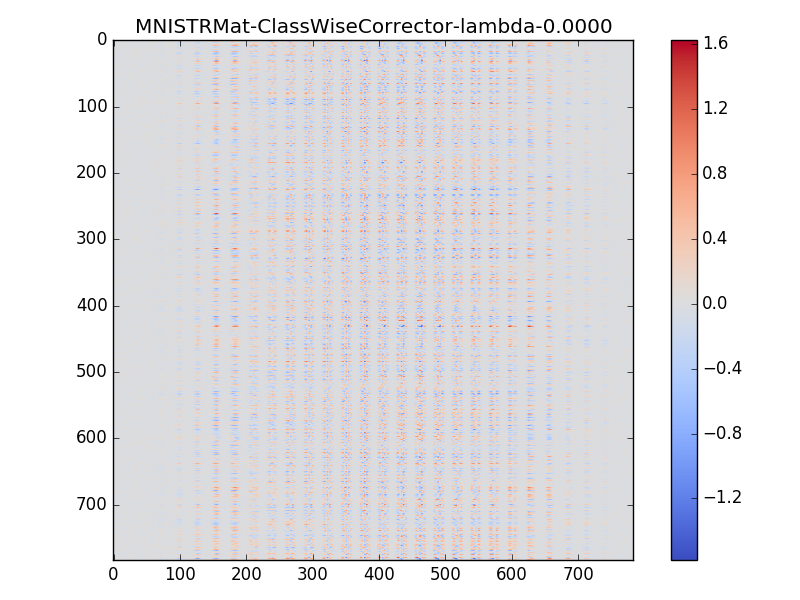
\includegraphics[width=0.45\linewidth]{fig/05-04-2016/MNISTRMat-ClassWiseCorrector-lambda-0.0000-Weights.png}}
\caption{MNIST - RMat correcteur non aligné}
\label{fig:mnist_rmat_classwise}
\end{figure}


%-----------------------------------------

\experiment{Corriger Moon après transformations linéaire}

Maintenant on passe sur des données à 2 dimensions. L'exemple des demi-lunes
(Moon) est un exemple non linéaire simple en 2D.

%----------------------------------------------------------------------------------------


\labday{Mercredi, 6 avril 2016}
\label{day:06-04-2016}

\experiment{Utiliser l'adversarial pour améliorer le correcteur}

\begin{figure}[H]
\centering
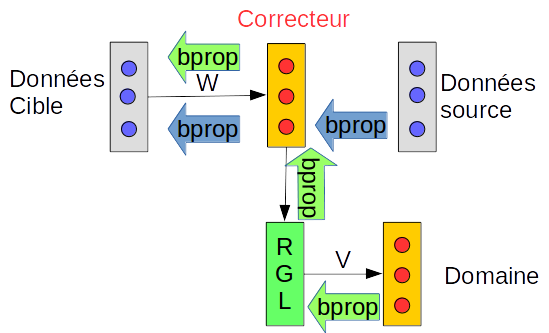
\includegraphics[width=0.45\linewidth]{fig/05-04-2016/Correcteur-Adversarial.png}
\caption{Correcteur adversarial}
\label{fig:correcteur_adversarial2}
\end{figure}

{\huge \textsc{Épic fail !}}

Non mais vraiment, ça marche pas du tout. Les résultats sont au mieux 
identiques (quand $\lambda_D\approx 0$) quelque soient les données que j'ai utilisées.


\experiment{Apprendre l'alignement}

Utiliser uniquement les classes pour déterminer l'alignement n'est pas suffisant.


%----------------------------------------------------------------------------------------


\labday{Lundi, 11 avril 2016}
\label{day:11-04-2016}

{\Large \textbf{Vocabulaire}}

L'objectif de ces expériences est d'arriver à associer entre-elles des données
provenant de distributions très similaires.

On dispose d'un jeu de donnée \textbf{Source} qui contient les données 
\textbf{Originales}, \textbf{Non biaisées} ou encore proviennent de
la \textbf{Réalité}.

Ce jeu de donnée est opposé aux données \textbf{Cible} qui contiennent des
données \textbf{Transformées}, \textbf{biaisées} ou encore proviennent de
\textbf{Simulations}.

On cherche ici à construire un \textbf{correcteur} qui va rapprocher/projeter
les données \emph{Cibles} sur les données \emph{Sources} correspondantes.

On note $\mathcal{X_S}$ les données sources, $\mathcal{X_T}$ les données 
cibles (Target) et $\mathcal{Y}$ les labels (s'il y en a).

On note $\phi$ la fonction inconnue qui a transformé/biaisé les données \emph{Cible}.
\begin{align*}
\phi : \mathcal{X_S}  &\to \mathcal{X_T} \\
                  x &\mapsto x^\prime
\end{align*}

Et $\psi$ la fonction que notre modèle va apprendre. On espère obtenir
$\phi \circ \psi = identity$.



\experiment{Apprendre l'alignement : résumé des idées et discussions}

Je résume ici une discussion sur les problèmes et solutions sur l'algorithme
visant à apprendre l'alignement pendant l'entraînement du correcteur.

\subexperiment{Brute Force}

Commençons par rappeler l'algo \emph{brute force} que l'on va par la suite
tenter d'améliorer.

L'idée précédente était d'utiliser les classes ou les sous-classes connues
afin de tenter d'aligner les données. 

\begin{algorithm}[tb]
   \caption{Alignement aléatoire}
   \label{alg:align_random}
\begin{algorithmic}
    \State {\bfseries Entrée:} données cible $\mathcal{X_T}$, données cibles $\mathcal{X_S}$, classes $\mathcal{Y}$
    \State \textcolor{gray}{Initialisation :}
    \State $c \gets $ nombre de classe dans $\mathcal{Y}$
    \State $n \gets $ nombre d'exemple dans $\mathcal{X_T}$
    \State $NN \gets$ réseau de neurone initialisé
    \While{Convergence ou temps écoulé}
        \State \textcolor{gray}{Réorganiser aléatoirement l'alignement en respectant les classes :}
        \State $idx \gets \text{array}(n)$
        \For{$i=0$ {\bfseries to} $c$}
            \State $idx_i \gets \text{where}(\mathcal{Y}=i)$
            \State $idx_i^\prime \gets \text{shuffle}(idx_i)$
            \State $idx[idx_i]\gets idx_i^\prime$
        \EndFor
        \State $\mathcal{X_T} \gets \mathcal{X_T}[idx]$
        \State \textcolor{gray}{Entraîner le réseaux pour 1 époque :}
        \State $NN.\text{train}(\mathcal{X}, \mathcal{X_S})$
    \EndWhile
    \State {\bfseries Rendre} le réseaux
\end{algorithmic}
\end{algorithm}

Cela permet en effet de ramener des distributions `en paquet' correctement 
(figure \ref{fig:cloud_rotated_classwise})

\begin{figure}[H] % images
\centering
\subfigure[Corrected data]
    {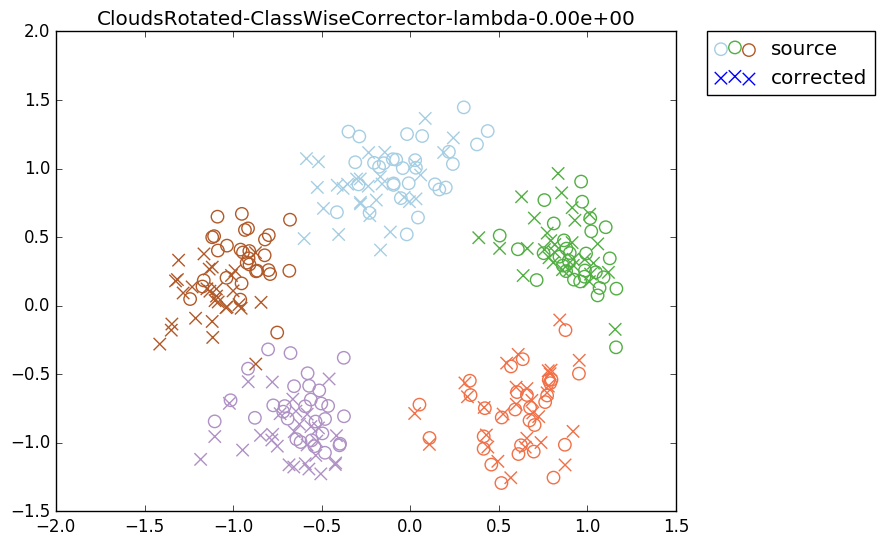
\includegraphics[width=0.45\linewidth]{fig/11-04-2016/CloudsRotated-ClassWiseCorrector-lambda-0.00e+00-corrected_data.png}}
\hfill
\subfigure[Target Data (uncorrected)]
    {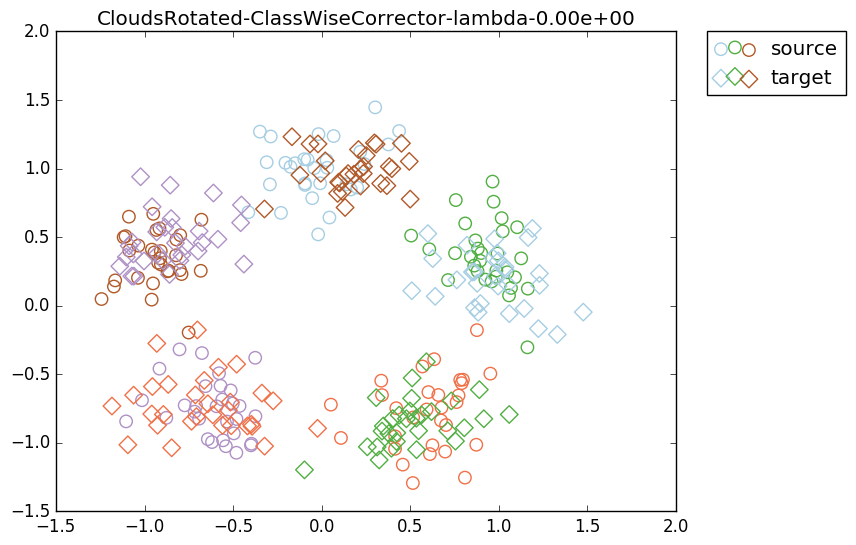
\includegraphics[width=0.45\linewidth]{fig/11-04-2016/CloudsRotated-ClassWiseCorrector-lambda-0.00e+00-target_data.png}}
\caption{Clouds - Rotated }
\label{fig:cloud_rotated_classwise}
\end{figure}


Cependant comme vu précédemment (section \ref{exp:moon_0}) dans le cas de
distribution qui ne sont pas de simples nuages de point `gentils' cette approche 
peut mener à écraser les données corrigées sur le centre des distributions.
L'idée est donc d'apprendre l'alignement afin de faire mieux que rapprocher les
données du centre des distributions Source.

Plutôt que d'aligner aléatoirement les données entre chaque époque on va chercher
les éléments de la \emph{Source} qui correspondent le plus ou sont plus proche de 
ceux provenant de la \emph{Cible}. Il nous faut donc une distance : 
$$ \Delta : x, x^\prime \mapsto distance(x, x^\prime)$$

La première idée d'algorithme serait de d'aligner les données \emph{Cibles} avec leur
plus proche voisin dans les données \emph{Sources}. Cependant une solution triviale
alignant tous les exemples de la \emph{Cible} sur un seul et même exemple de la 
\emph{Source} est à éviter.

Pour éviter cette solution il faut forcer les exemples de la \emph{Cible} à s'aligner 
sur des exemples différents de la \emph{Source}.
On considère donc les $k$ plus proches voisins de chaque élément $x_T$ de la \emph{Cible}
Puis on l'aligne sur le plus proche voisin qui a été le moins choisis jusqu'à présent.


\begin{algorithm}[tb]
   \caption{Alignement KNN (K Nearest Neighbors)}
   \label{alg:align_KNN}
\begin{algorithmic}
    \State {\bfseries Entrée:} données cible $\mathcal{X_T}$, données cibles $\mathcal{X_S}$, classes $\mathcal{Y}$
    
    \Function{k-closest}{$x, X_S$} 
    \State $n \gets $ nombre d'exemple dans $\mathcal{X_S}$
    \State $closest \gets \text{array}(n)$
    \For{$i=0$ {\bfseries to} $n$}
        \State $closest[i] \gets \Delta(x, X_S[i])$
    \EndFor           
    \EndFunction

    \State \textcolor{gray}{Initialisation :}
    \State $c \gets $ nombre de classe dans $\mathcal{Y}$
    \State $n \gets $ nombre d'exemple dans $\mathcal{X_T}$
    \State $NN \gets$ réseau de neurone initialisé
    \While{Convergence ou temps écoulé}
        \State \textcolor{gray}{Réorganiser aléatoirement l'alignement en respectant les classes :}
        \State $idx \gets \text{array}(n)$
        \For{$i=0$ {\bfseries to} $c$}
            \State $idx_i \gets \text{where}(\mathcal{Y}=i)$
            \For{$j=0$ {\bfseries to} $n$}
                \State $closest \gets \textsc{k-closest}(\mathcal{X_T}[j], \mathcal{X_T})$
            \EndFor
            \State $idx[idx_i]\gets idx_i^\prime$
        \EndFor
        \State $\mathcal{X_T} \gets \mathcal{X_T}[idx]$
        \State \textcolor{gray}{Entraîner le réseaux pour 1 époque :}
        \State $NN.\text{train}(\mathcal{X_T}, \mathcal{X_S})$
    \EndWhile
    \State {\bfseries Rendre} le réseaux
\end{algorithmic}
\end{algorithm}


Cet algorithme est malheureusement quadratique au moment du calcul de la 
matrice de distance deux à deux entre les données \emph{Source} et \emph{Cible}.
Même si ce calcul peut être parallélisé, il reste particulièrement lourd.


\subexperiment{Les clusters (vivent les k-means !)}

1) $\psi : \text{source} \mapsto \text{cible}$

2) (Hypothèse 1) Source distribué en mixture poids différents

- Si $\psi$ est sympathique alors \emph{cible} est aussi distribué en mixture

$x_i$, centre des distributions sources
$x_j$, centre des distributions cible

init :
$$\phi : x_i \mapsto x_j$$
$$card(C_i) \approx card(C_j)$$
où $C_i$ est l'ensemble des exemples rattachés au centre $i$

- Si (Hypothèse 1) ne tient pas, alors on utilise un argument de simplicité pour 
sélectionner (désambiguïser).

Supposons une série de clusters de centres $z_1, ..., z_k$ et de poids (probabilité)
$p_1, ... p_k$ formant la distribution \emph{source}.

$$\phi : x^\prime \mapsto i, |\phi(x^\prime) - z_i| + c |p_i-p_i^\prime|$$



%----------------------------------------------------------------------------------------


\labday{Jeudi, 21 avril 2016}
\label{day:21-04-2016}

Je vais résumer ici l'avancement du projet d'apprendre l'alignement,
les problèmes rencontrés et les solutions auxquelles on a pensé.

{\Large \textbf{Vocabulaire}}

L'objectif de ces expériences est d'arriver à associer entre-elles des données
provenant de distributions très similaires.

On dispose d'un jeu de donnée \textbf{Source} qui contient les données 
\textbf{Originales}, \textbf{Non biaisées} ou encore proviennent de
la \textbf{Réalité}.

Ce jeu de donnée est opposé aux données \textbf{Cible} qui contiennent des
données \textbf{Transformées}, \textbf{biaisées} ou encore proviennent de
\textbf{Simulations}.

On cherche ici à construire un \textbf{correcteur} qui va rapprocher/projeter
les données \emph{Cibles} sur les données \emph{Sources} correspondantes.

On note $\mathcal{X_S}$ les données sources, $\mathcal{X_T}$ les données 
cibles (Target) et $\mathcal{Y}$ les labels (s'il y en a).

On note $\phi$ la fonction inconnue qui a transformé/biaisé les données \emph{Cible}.
\begin{align*}
\phi : \mathcal{X_S}  &\to \mathcal{X_T} \\
                  x &\mapsto x^\prime
\end{align*}

Et $\psi$ la fonction que notre modèle va apprendre. On espère obtenir
$\phi \circ \psi = identity$.


\experiment{Algo exhaustif}

\textbf{\large Rappel :} l'algo exhaustif cherche les $k$ plus proches voisins
de chaque point parmi les données \emph{Source} et les données 
\emph{Corrigées} (\emph{Cible} après correction). Puis choisit parmi ces $k$ 
plus proche voisin le voisin qui a été le moins choisi jusqu'à présent.

Le défaut principal de l'algorithme exhaustif se fait ressentir sur les données
aux distributions plus subtiles (par exemple les demi-lunes que l'on va étudier ici) 
qu'une distribution gaussienne. Le réseaux de neurone est vite coincé dans un
état où on lui demande de reconstruire les points de la \emph{Source} en lui 
donnant les mauvais points de la \emph{Cible}, ce qu'il ne peut pas résoudre.

Cela se traduit par un ratatinement des données après corrections (figure \ref{fig:exhaustive-pb}).

\begin{figure}[H] % images
\centering
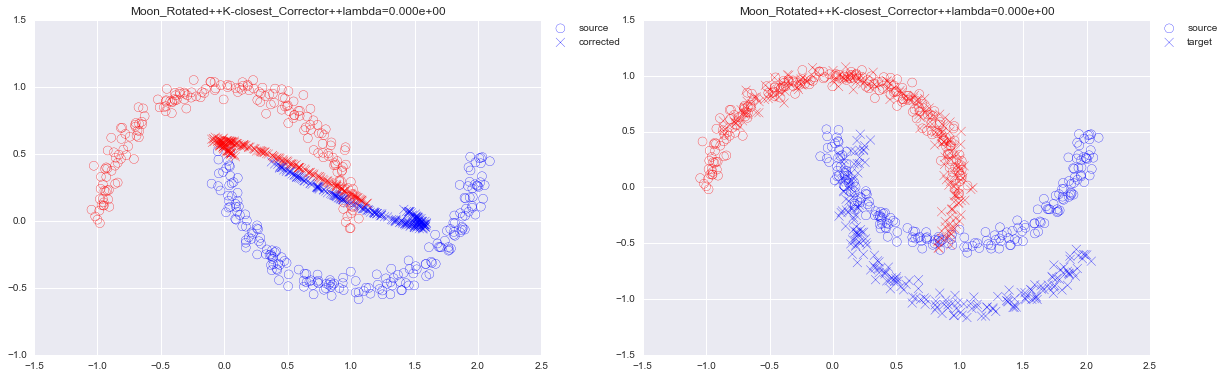
\includegraphics[width=\linewidth]{fig/21-04-2016/exhaustive-pb.png}
\caption{Correction sous contrainte de dé-correction possible}
\label{fig:exhaustive-pb}
\end{figure}

Une piste possible pour éviter cet écrasement des données serait de forcer le 
réseaux à ne pas perdre de l'information en lui demandant de reconstruire les
données \emph{Cible} après leurs corrections (figure \ref{fig:de-correcteur}).

\begin{figure}[H] % images
\centering
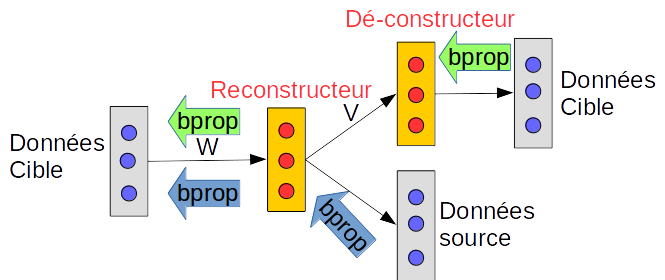
\includegraphics[width=0.45\linewidth]{fig/21-04-2016/Re-De-constructeur.png}
\caption{Correction sous contrainte de dé-correction possible}
\label{fig:de-correcteur}
\end{figure}

Voir même, rêvons un peu, rendre cette partie récurrente (figure \ref{fig:recurrent-de-correcteur}).
\begin{figure}[H] % images
\centering
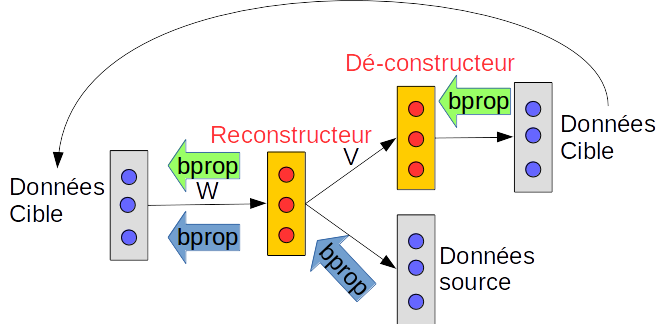
\includegraphics[width=0.45\linewidth]{fig/21-04-2016/Recurrent-correcteur.png}
\caption{Correction sous contrainte de dé-correction possible, version récurrente}
\label{fig:recurrent-de-correcteur}
\end{figure}

Enfin le temps de calcul ne passe pas à l'échelle (complexité $\mathcal O (n^2)$).
Malgré la parallélisation avec GPU, sur MNIST la plupart du temps de calcul 
est alloué aux calculs des distances 2 à 2 (150 sec par époque contre 1.5 sec 
pour le NN).

Cette méthode est aussi trop sensible à l'initialisation. En fait elle 
requiert que l'initialisation résolve le problème.

\experiment{K-moyennes}

Pour palier au problème de l'algo exhaustif on peut construire des clusters. 
Puisque le problème est résolu pour les simples nuages de points, il suffit 
de se ramener à ce problème. On va donc sous-diviser les données \emph{Sources}
et les données \emph{Cible} en petits paquets à l'aide de K-moyennes.

Intérêts:
\begin{enumerate}
	\item Le calcul des distances 2 à 2 reste quadratique mais sur un petit 
	nombre de points. Donc faisable.
	\item On va ainsi capturer les formes des distributions plus complexes (si
	on donne suffisamment de clusters).
\end{enumerate}

\textbf{Notations :} (Les notations de la section précédente n'étaient pas très intuitive)
\begin{description}
\item[$S_i$] les clusters de la distribution \emph{Source} 
	($S_i \subset \mathcal X_S$)
\item[$s_i$] les centres des clusters de la distribution \emph{Source} 
\item[$C_i$] les clusters de la distribution \emph{Cible} 
	($C_i \subset \mathcal X_T (= \phi(\mathcal X_S)$)
\item[$c_j$] les centres des clusters de la distribution \emph{Cible}  
\item[$C_i^\prime$] les clusters de la distribution \emph{Corrigée} 
	($C_i^\prime \subset \mathcal \psi(\mathcal X_T) )$ 
\item[$c_j^\prime$] les centres des clusters de la distribution \emph{Corrigée}
\end{description}

Remarques :

Si $\phi$ ne change pas les distances alors on peut raisonnablement 
espérer (démo ?) qu'il existe une association $c_j = \phi(s_i)$. Cependant il 
est toujours vrai que $c_j^\prime = \psi(c_j)$ par définition.


Maintenant nous allons nous pencher sur les problèmes de cette méthode et 
les solutions possibles.


\subexperiment{Ambiguïté}

Nous utilisons donc 2 K-moyennes, un pour construire $k$ clusters dans la 
distribution \emph{Source} (notés $S_i$) et un pour construire $k$ clusters
dans la distribution \emph{Cible} (noté $C_i$). Ces derniers servent à
obtenir des clusters $C_i^\prime = \psi(C_i)$ en passant les points de $C_i$
dans le \emph{correcteur} (ici un réseau de neurone).

Je pensais ce problème analogue à celui des nuages de points qui fonctionnait
très bien. En fait NON. On ignore quel cluster $C_i$ va avec quel cluster
$S_i$ contrairement aux nuages de points où on connaissait déjà cet alignement !

On arrive donc au premier problème, \textbf{l'ambiguïté}. Le \emph{correcteur}
se retrouve bloqué si il se trompe sur l'alignement de certain cluster.

\begin{figure}[H] % images
\centering
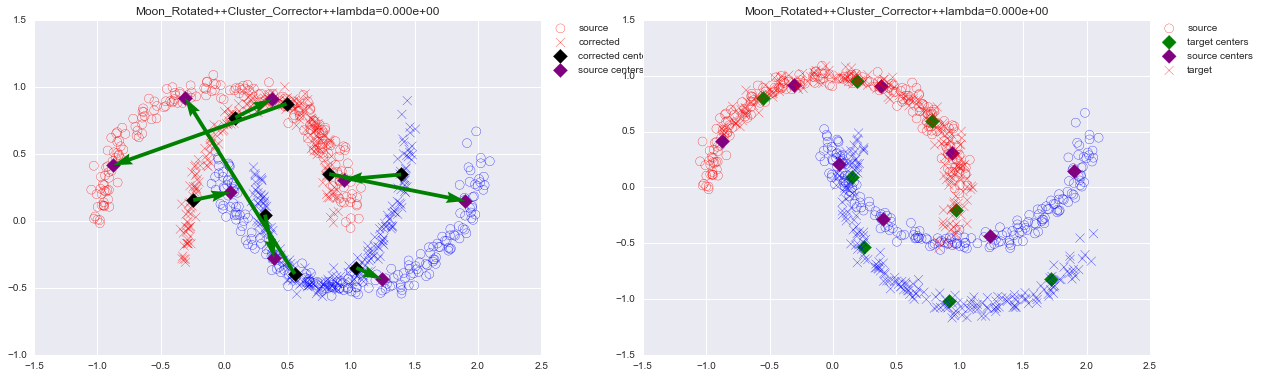
\includegraphics[width=\linewidth]{fig/21-04-2016/stuck_blue-red.png}
\caption{Ambiguïté du choix de l'alignement}
\label{fig:stuck_red_blue}
\end{figure}
On observe sur la figure \ref{fig:stuck_red_blue} que les clusters corrigés 
(en noir) sont alignés (flèches) sur les mauvais clusters sources (en violet).
Ce problème bloque le correcteur dans un état ``tiraillé'' ou ``oscillant''.
On observe une ``oscillation'' (ça vibre quoi) des données corrigées quand 
on regarde chaque époque l'une après l'autre.

Ce problème peut être absorbé par l'utilisation des classes. Ici les deux 
lunes sont ``interchangeables'', une solution à l'alignement pourrait être 
de mettre les bleus sur les rouges et les rouges sur les bleus.
Utiliser les classes (information dont on dispose après tout) peut 
désambiguïser. Enfin presque ! Dans le cas de la figure \ref{fig:stuck_2}
on a une seule erreur (permutation de 2 clusters) qui empêche le correcteur
d'atteindre un résultat parfait.

\begin{figure}[H] % images
\centering
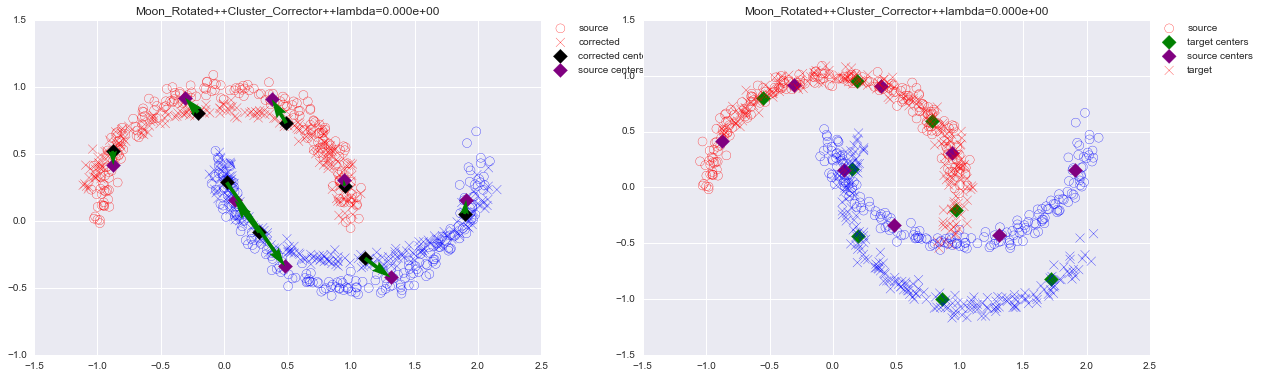
\includegraphics[width=\linewidth]{fig/21-04-2016/Stuck_2.png}
\caption{Ambiguïté du choix de l'alignement}
\label{fig:stuck_2}
\end{figure}


\subexperiment{Initialisation}

Ces derniers résultats sont assez encourageant. Cependant ils ont été obtenus
après moult essais. En effet la méthode est très sensible à l'initialisation.

\textcolor{red}{Erratum} : les expériences de Lundi, 25 avril matin montre que 
l'initialisation ne pose plus vraiment de problème pour le problème des 
demi-lunes. Si on utilise suffisamment de clusters (4) le correcteur réussit 
au bout de quelques époques.
Cependant trop de cluster tue l'efficacité du correcteur (ambiguïté) exemple
figure \ref{fig:stuck_trop}.

\begin{figure}[H] % images
\centering
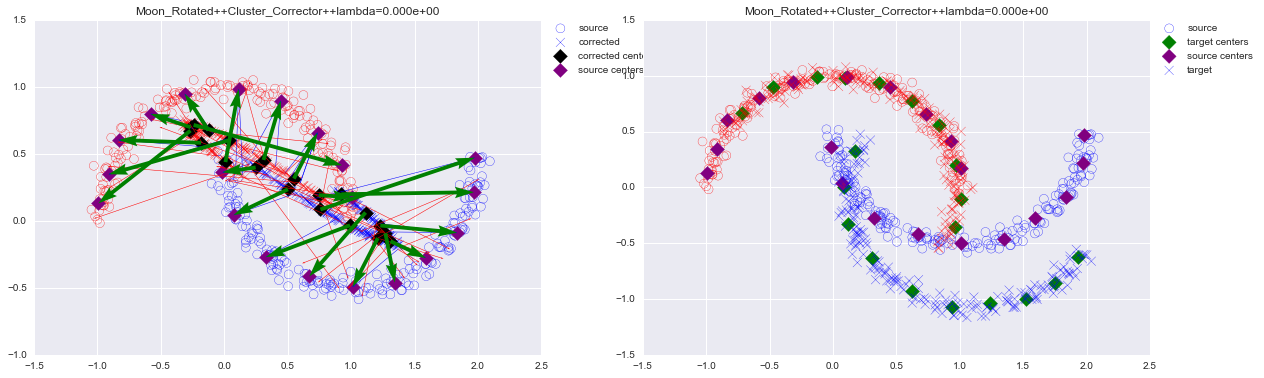
\includegraphics[width=\linewidth]{fig/21-04-2016/Stuck_trop.png}
\caption{Ambiguïté du choix de l'alignement}
\label{fig:stuck_trop}
\end{figure}

Bref. L'initialisation reste probablement un problème clé pour l'entraînement 
du correcteur, une mauvaise initialisation pouvant amener à des cas 
pathologiques.

Solutions : 
\begin{enumerate}
	\item Lancer 50 initialisations et prendre la meilleure, ce qui requiert
une mesure fine de la performance de la correction.
	\item Initialiser proche de l'identité, cela requiert l'hypothèse que 
la solution en est proche. Cela reste une méthode pour utiliser les 
connaissances expertes sur le problème. De plus elle est compatible avec
la précédente.
\end{enumerate}

% TODO : 
\subexperiment{Autres}

Quid du cas où $\phi$ ajoute ou divise des distributions ? Dans ce cas le 
correcteur ne doit pas simplement renvoyer un point sur un autre mais aussi 
discriminer les points importants des parasites. De plus l'hypothèse de $\phi$
conservant les distances ne tient plus.
(faire un exemple avec Clouds)

Créer de nouveaux toys ! Si on avait pas utilisé les Moons j'aurais raté 
pleins de problèmes ! Qui sait ce qu'on rate encore ? De façons générale il 
faut tester les limites de la méthode et trouver des moyens pour diagnostiquer
les cas pathologiques pour appliquer les bonnes corrections.

\begin{figure}[H] % images
\centering
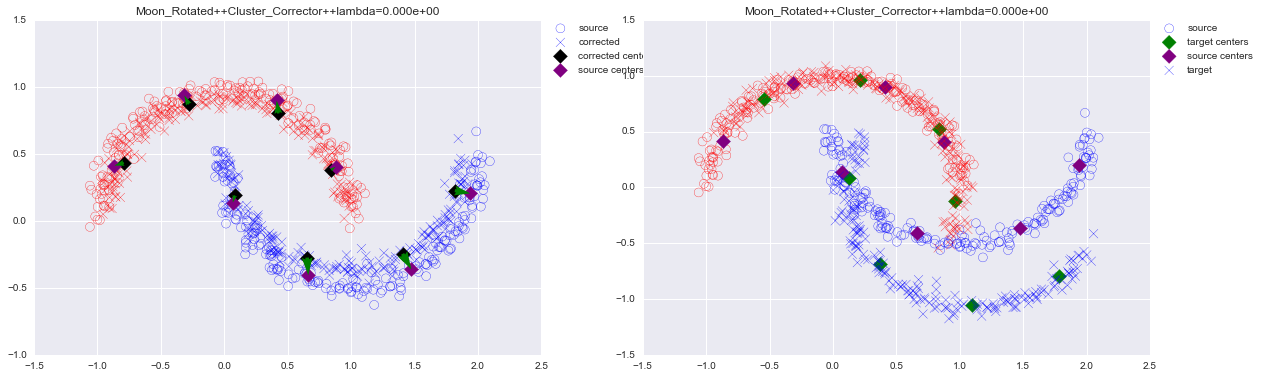
\includegraphics[width=\linewidth]{fig/21-04-2016/good_init.png}
\caption{Quand ça marche}
\label{fig:good_init}
\end{figure}


\subexperiment{Résumé des Pistes}
\begin{enumerate}
	\item Mesure plus fine des performances du correcteur. KL, comparaison des
	histogrammes des clusters, de leur variance à inclure dans la distance
	\item Initialisation multiple + choix de la meilleure.
	\item Initialiser selon les connaissances expertes (à l'identité par exemple)
	\item Créer de nouveau Toys pour tester la robustesse de la méthode face 
	à divers types de transformation.
	\item Rendre le choix de l'alignement des clusters moins déterministe 
	(pour éviter figure \ref{fig:stuck_2})
\end{enumerate}


%----------------------------------------------------------------------------------------


\labday{Mardi, 24 mai 2016}
\label{day:24-05-2016}

Aujourd'hui, je vais rassembler l'intégralité des résultats dans ce cahier.
Tous les toys, toutes les transformations linéaires et même un petit bonus avec
la grille tordue !

L'objectif étant de faire une compilation des expérimentations faites jusqu'à présent
avec le correcteur linéaire.

\experiment{Rappels}

L'objectif de ces expériences est d'arriver à associer entre-elles des données
provenant de distributions très similaires.

\begin{itemize}
	\item $\mathcal{X_S}$: données \textbf{Sources} \textbf{Originales}, \textbf{Non biaisées}, \textbf{Réalité}.
	\item $\mathcal{X_T}$: données \textbf{Cible}, \textbf{Transformées}, \textbf{biaisées}, \textbf{Simulations}.
	\item $\phi$: la \textbf{transformation}, le \textbf{biais}
	\item $\psi$: le \textbf{correcteur}, un réseau de neurone
\end{itemize}
On cherche : $\phi \circ \psi = identity$.

\textbf{L'alignement} est l'information qu'un point $x_i$ des données \emph{Sources} correspond 
à $x_i^\prime$ des données \emph{Cibles}. Cette information n'étant pas nécessairement 
disponnible dans les cas réels, on étudit les méthodes avec et sans cette information. 


Dans la suite je vais rassembler les résultats d'expérimentations par:
\begin{itemize}
	\item Jeu de donnée
	\begin{itemize}
		\item Méthode d'alignement
		\begin{itemize}
			\item Transformation
		\end{itemize}
	\end{itemize}
\end{itemize}
%%%%%%%%%%%%%%%%%%%%%%%%%%%%%%%%%%%%%%%%%%%%%%%%%%%%%%%%%%%%%%%%%%%%%%%%%%%%%%
%%%%%% CLOUDS
%%%%%%%%%%%%%%%%%%%%%%%%%%%%%%%%%%%%%%%%%%%%%%%%%%%%%%%%%%%%%%%%%%%%%%%%%%%%%%

\experiment{Clouds}

\emph{Clouds} est un jouet composé de $n$ classes (nuages de point gaussiens) se partageant 
l'espace sur le cercle unité.

Toutes ces expériences ont été réalisées avec un learning rate de $0.1$ + un moment de $0.9$.


\subexperiment{Alignement connu}

Le cas où l'alignement est connu permet de vérifier que la transformation est facile ou non 
à inverser, les autres méthode ayant peu de chance de faire mieux.

{\Large \textbf{Rotation :}}  On applique une rotation de 35 degrés par rapport à l'origine $(0,0)$.

\begin{figure}[H] % images
\centering
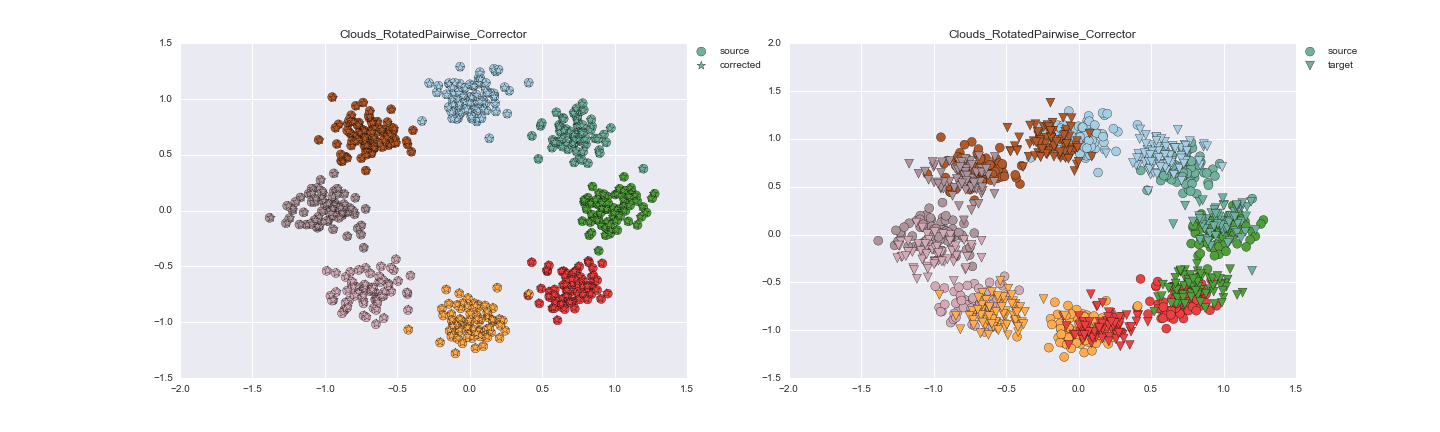
\includegraphics[width=\linewidth]{fig/24-05-2016/clouds/Clouds_RotatedPairwise_Corrector-DATA.png}
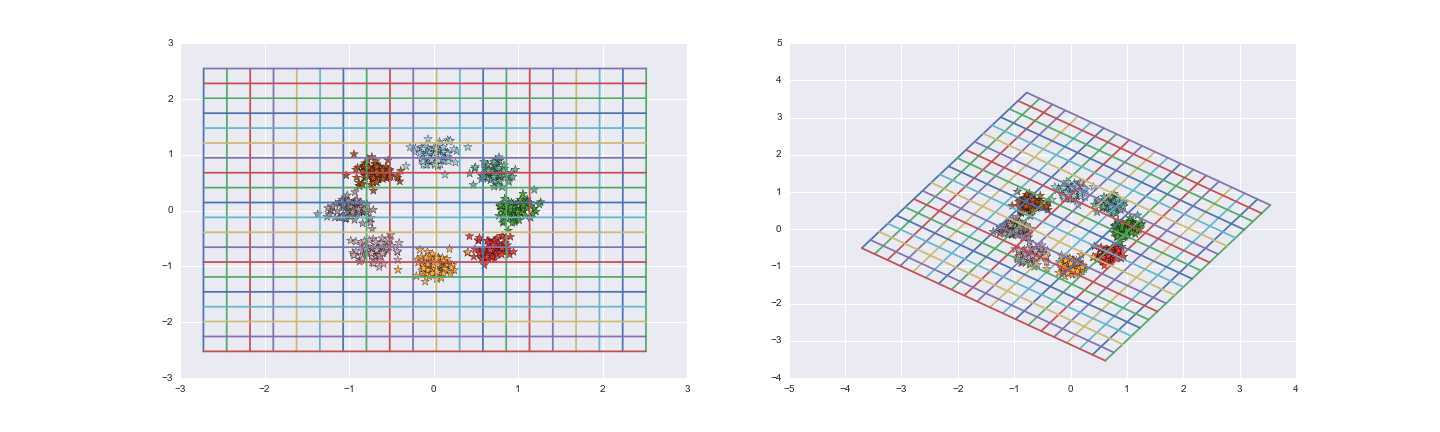
\includegraphics[width=\linewidth]{fig/24-05-2016/clouds/Clouds_RotatedPairwise_Corrector-GridCheck.png}
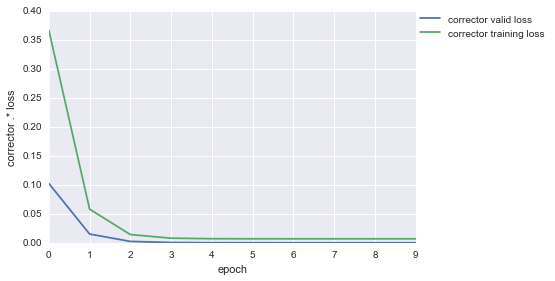
\includegraphics[width=0.45\linewidth]{fig/24-05-2016/clouds/Clouds_RotatedPairwise_Corrector-Learning_curve.png}
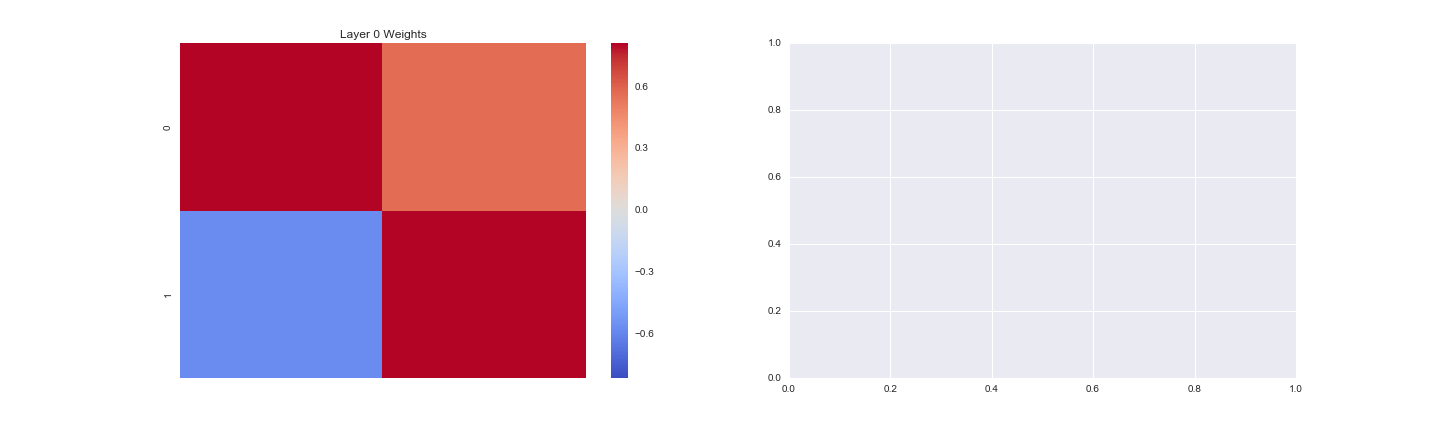
\includegraphics[width=\linewidth]{fig/24-05-2016/clouds/Clouds_RotatedPairwise_Corrector-W.png}
\caption{Correction de Clouds après une rotation de 35 degrés par rapport à l'origine avec alignement connu}
\label{fig:recap-clouds-rot-pairwise}
\end{figure}

{\Large \textbf{Random matrix :}}

\begin{figure}[H] % images
\centering
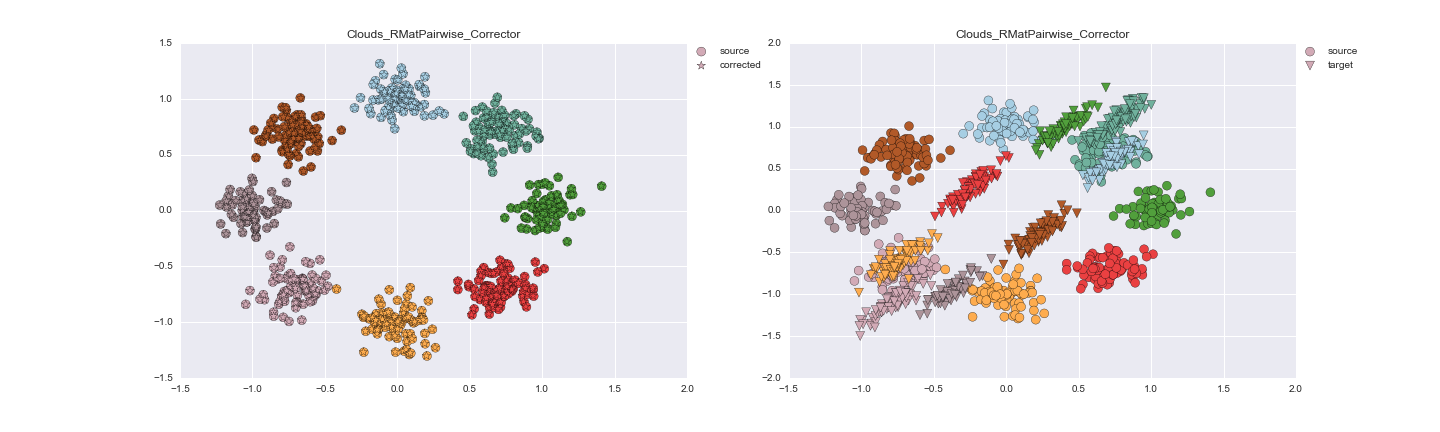
\includegraphics[width=\linewidth]{fig/24-05-2016/clouds/Clouds_RMatPairwise_Corrector-DATA.png}
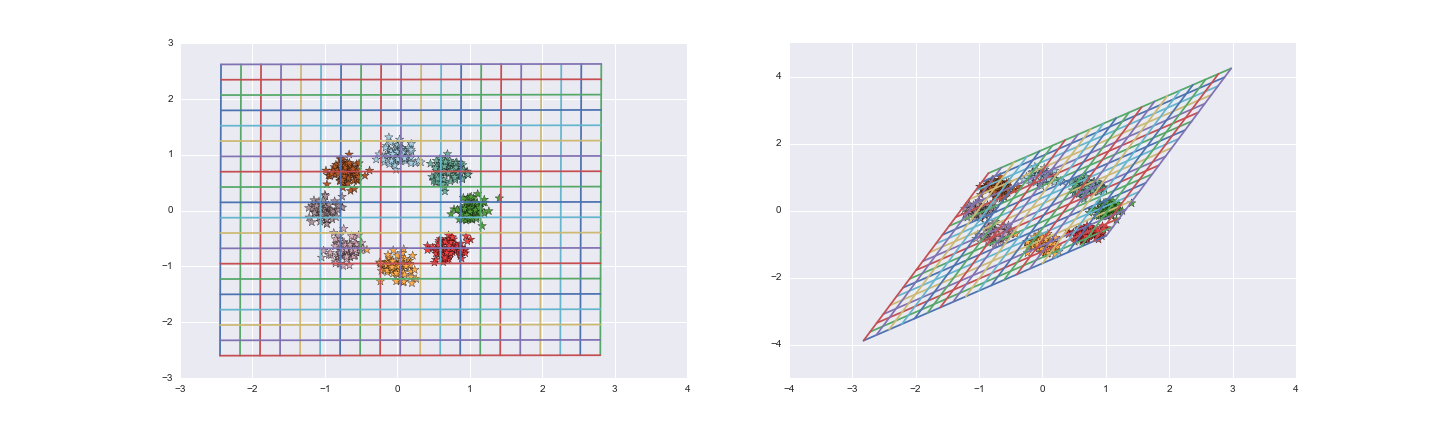
\includegraphics[width=\linewidth]{fig/24-05-2016/clouds/Clouds_RMatPairwise_Corrector-GridCheck.png}
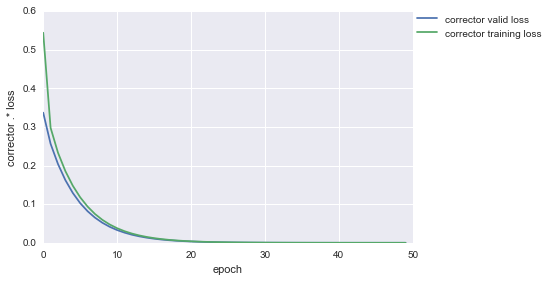
\includegraphics[width=0.45\linewidth]{fig/24-05-2016/clouds/Clouds_RMatPairwise_Corrector-Learning_curve.png}
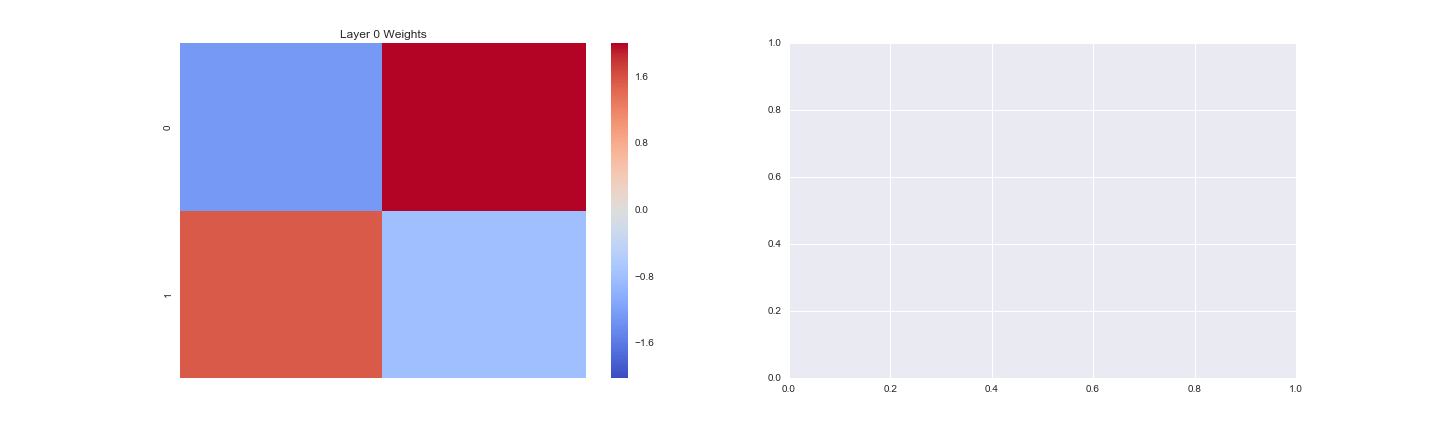
\includegraphics[width=\linewidth]{fig/24-05-2016/clouds/Clouds_RMatPairwise_Corrector-W.png}
\caption{Correction de Clouds après multiplication par une matrice générée aléatoirement}
\label{fig:recap-clouds-RMat-pairwise}
\end{figure}


{\Large \textbf{Grille tordue :}}

\begin{figure}[H] % images
\centering
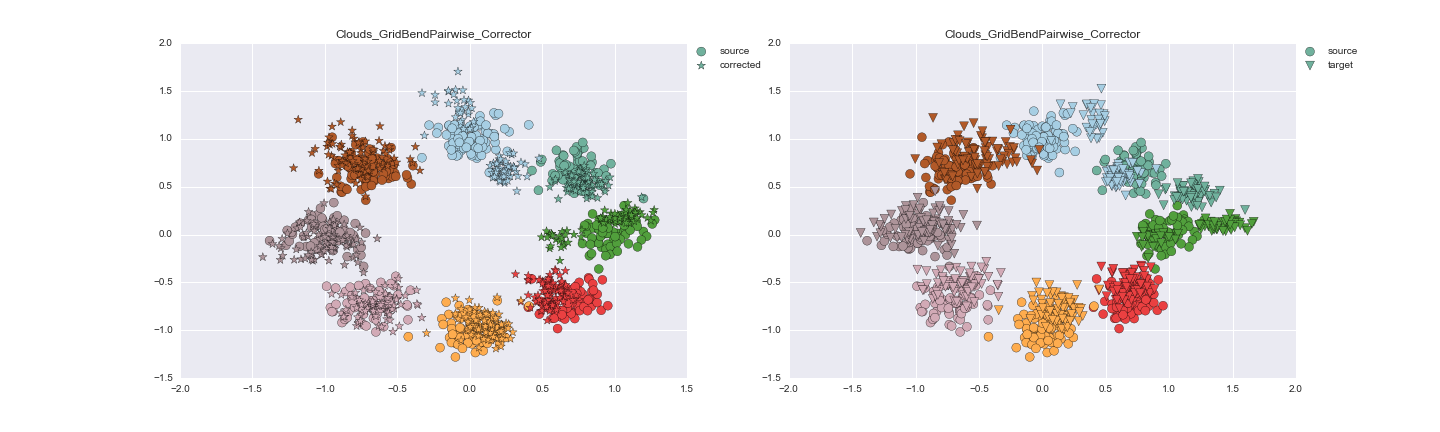
\includegraphics[width=\linewidth]{fig/24-05-2016/clouds/Clouds_GridBendPairwise_Corrector-DATA.png}
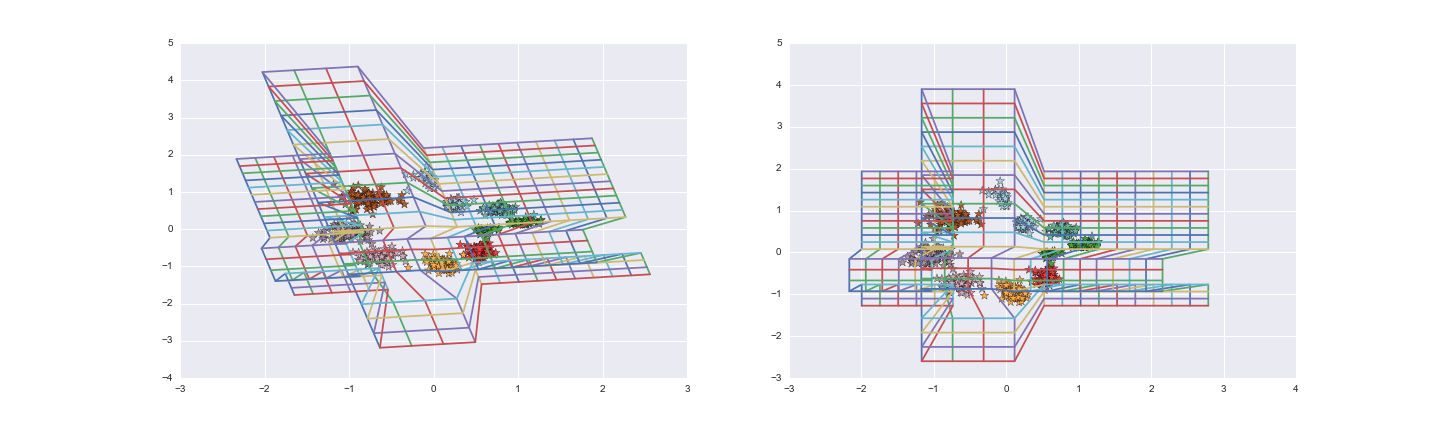
\includegraphics[width=\linewidth]{fig/24-05-2016/clouds/Clouds_GridBendPairwise_Corrector-GridCheck.png}
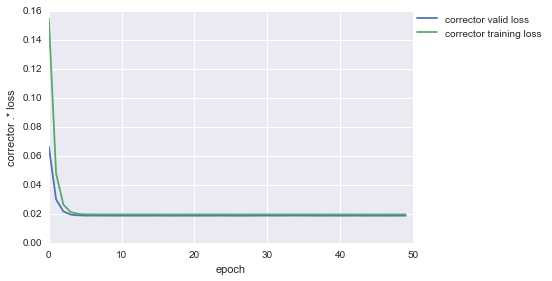
\includegraphics[width=0.45\linewidth]{fig/24-05-2016/clouds/Clouds_GridBendPairwise_Corrector-Learning_curve.png}
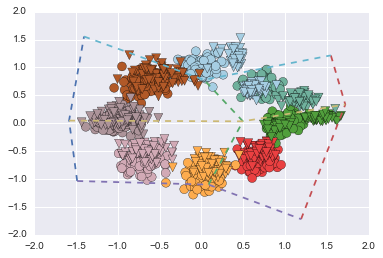
\includegraphics[width=0.45\linewidth]{fig/24-05-2016/clouds/cloud_grid.png}
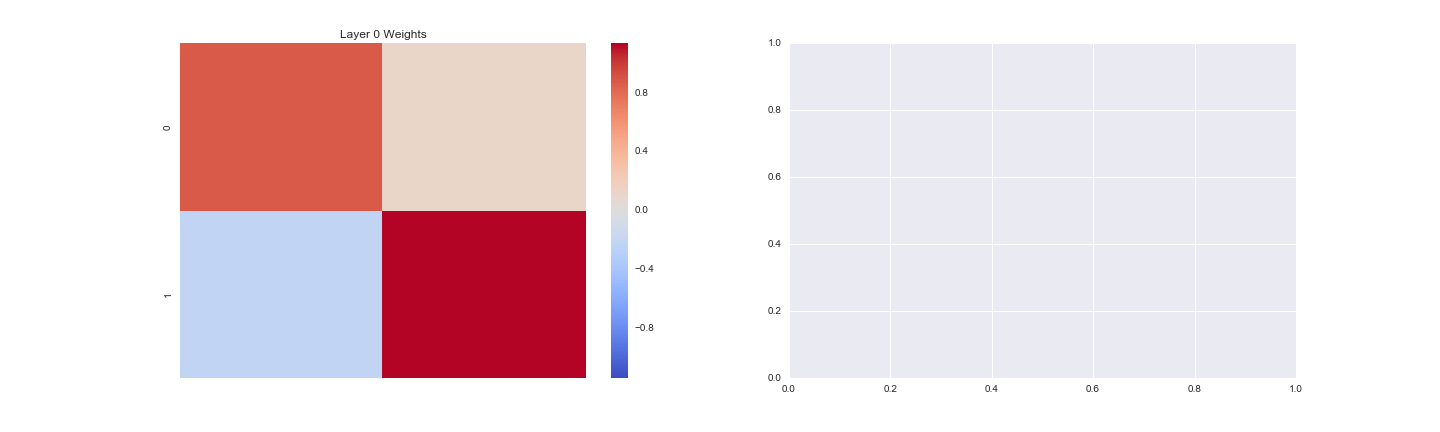
\includegraphics[width=\linewidth]{fig/24-05-2016/clouds/Clouds_GridBendPairwise_Corrector-W.png}
\caption{Correction de Clouds après application d'une transformation linéaire locale}
\label{fig:recap-clouds-GridBend-pairwise}
\end{figure}

\subexperiment{Alignement appris : alignement aléatoire au sein des classes}

{\Large \textbf{Rotation :}} On applique une rotation de 35 degrés par rapport à l'origine $(0,0)$.

\begin{figure}[H] % images
\centering
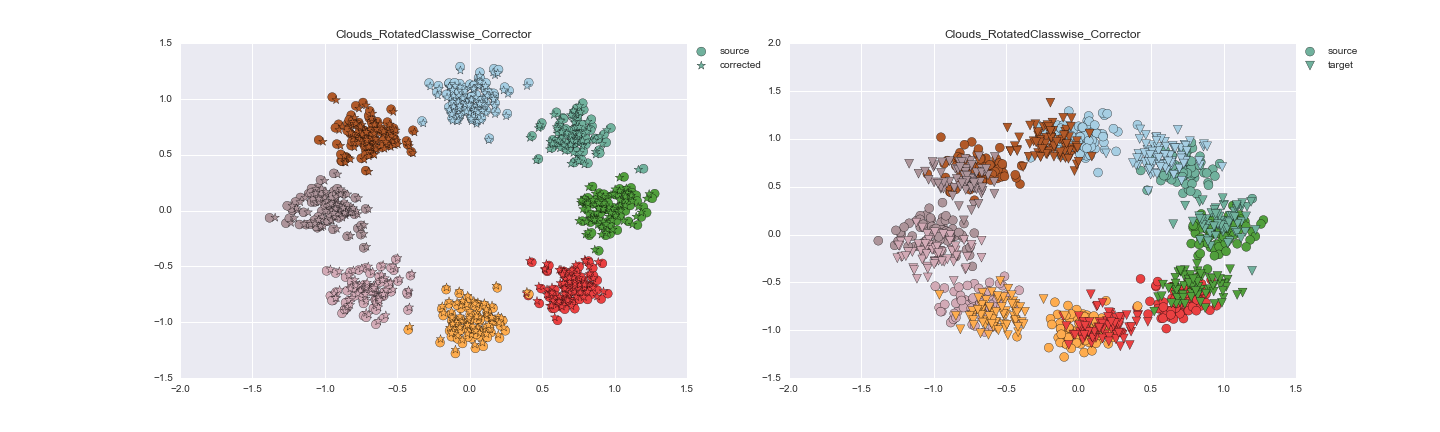
\includegraphics[width=\linewidth]{fig/24-05-2016/clouds/Clouds_RotatedClasswise_Corrector-DATA.png}
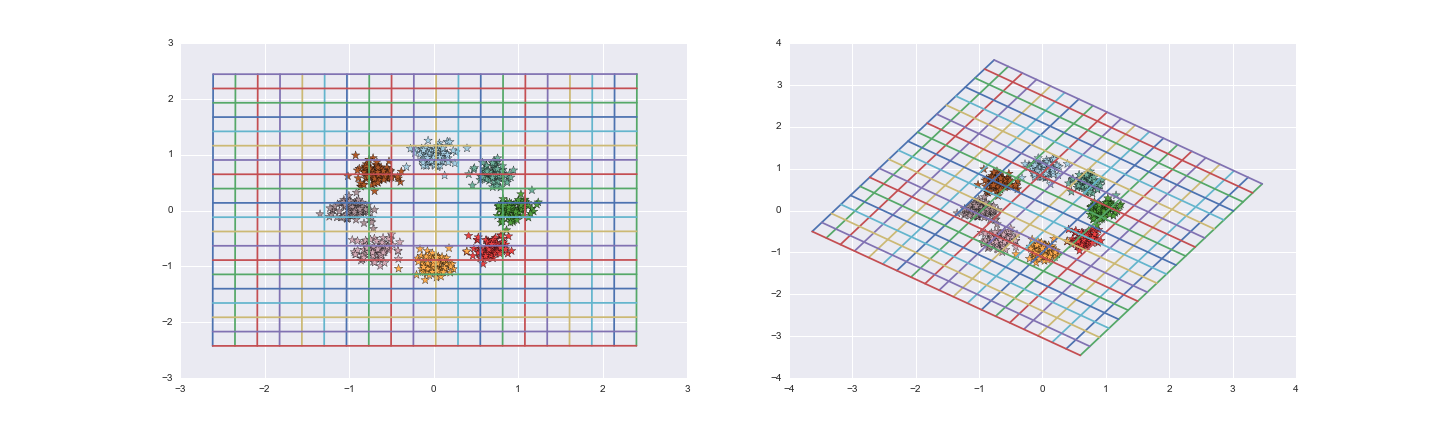
\includegraphics[width=\linewidth]{fig/24-05-2016/clouds/Clouds_RotatedClasswise_Corrector-GridCheck.png}
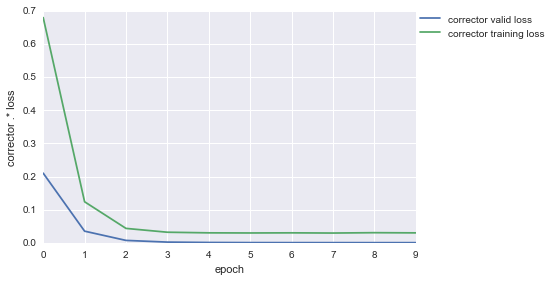
\includegraphics[width=0.45\linewidth]{fig/24-05-2016/clouds/Clouds_RotatedClasswise_Corrector-Learning_curve.png}
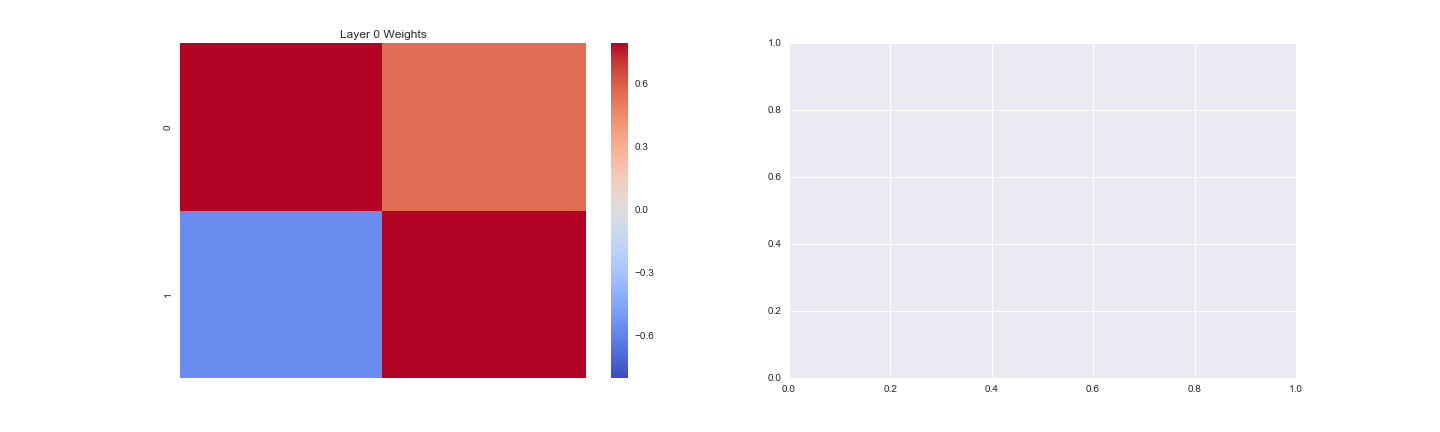
\includegraphics[width=\linewidth]{fig/24-05-2016/clouds/Clouds_RotatedClasswise_Corrector-W.png}
\caption{Correction de Clouds après une rotation de 35 degrés par rapport à l'origine avec les plus proches voisins entre les clusters}
\label{fig:recap-clouds-rot-classwise}
\end{figure}

{\Large \textbf{Random matrix :}}

\begin{figure}[H] % images
\centering
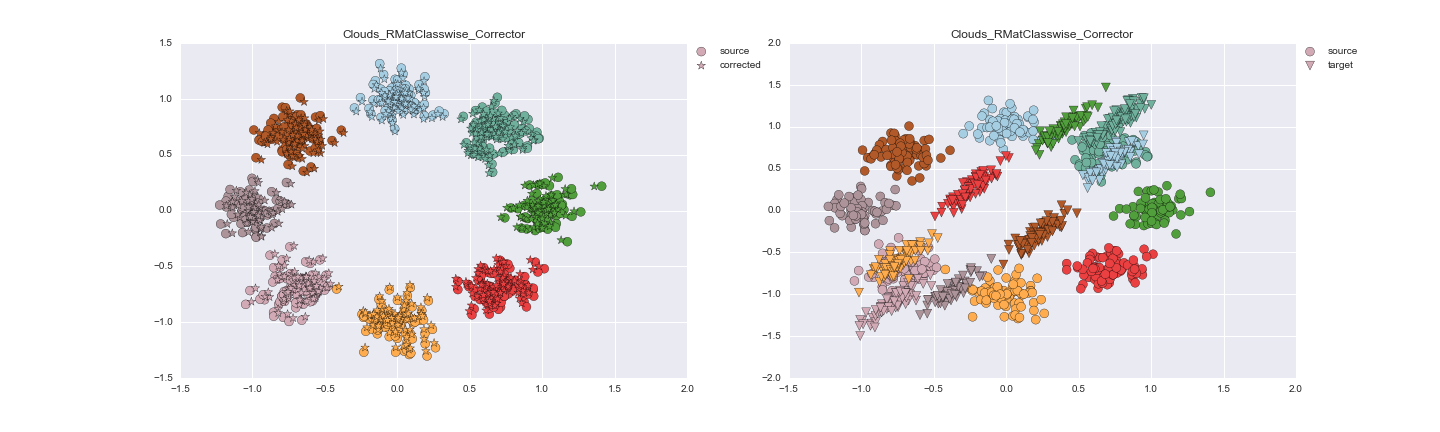
\includegraphics[width=\linewidth]{fig/24-05-2016/clouds/Clouds_RMatClasswise_Corrector-DATA.png}
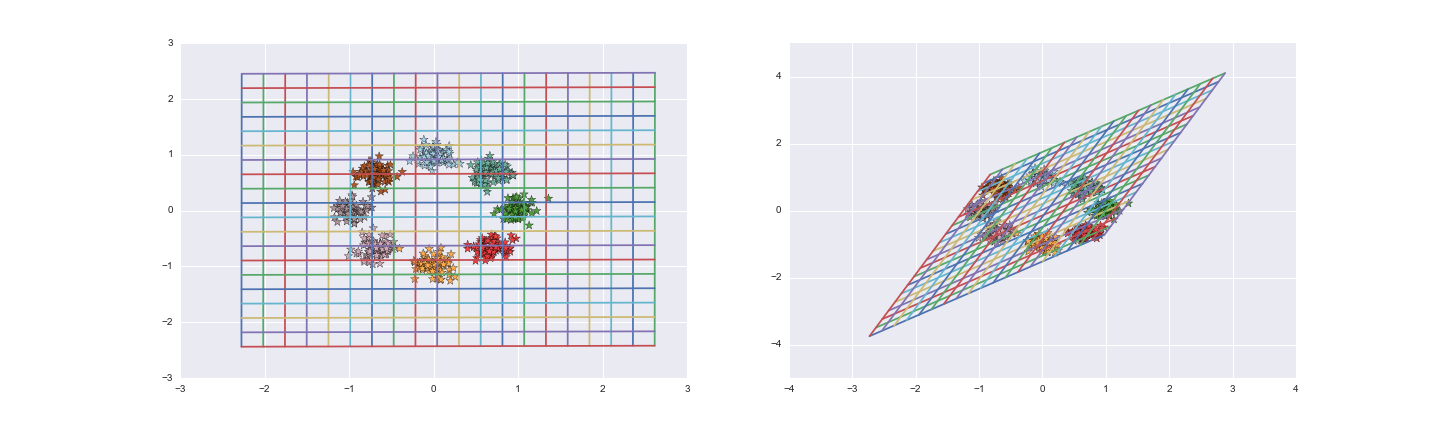
\includegraphics[width=\linewidth]{fig/24-05-2016/clouds/Clouds_RMatClasswise_Corrector-GridCheck.png}
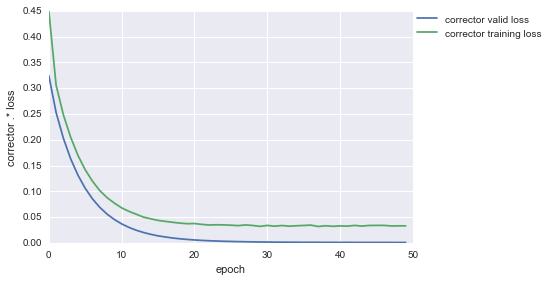
\includegraphics[width=0.45\linewidth]{fig/24-05-2016/clouds/Clouds_RMatClasswise_Corrector-Learning_curve.png}
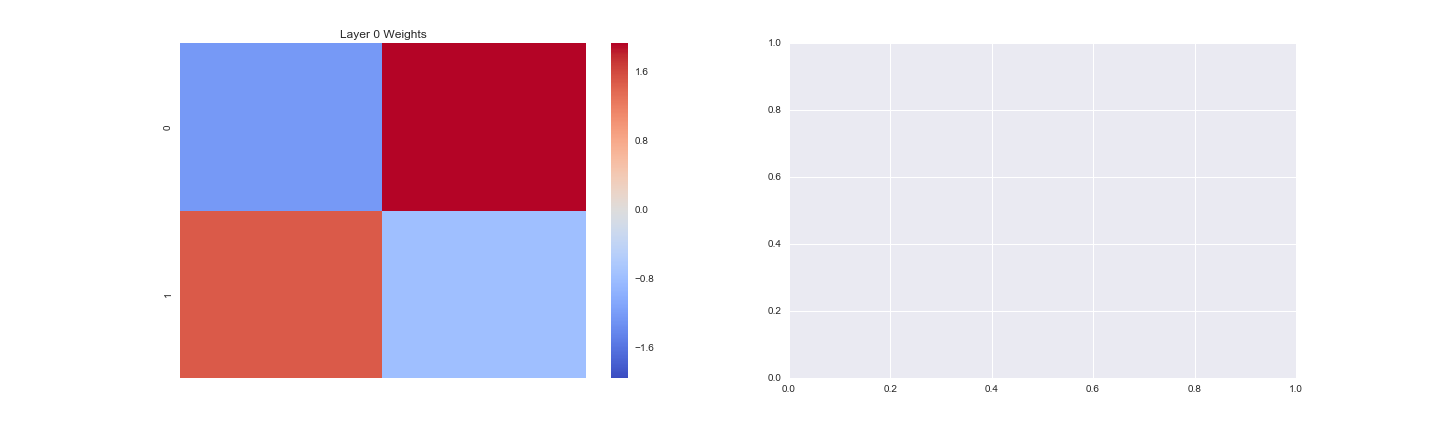
\includegraphics[width=\linewidth]{fig/24-05-2016/clouds/Clouds_RMatClasswise_Corrector-W.png}
\caption{Correction de Clouds après multiplication par une matrice générée aléatoirement}
\label{fig:recap-clouds-RMat-classwise}
\end{figure}

{\Large \textbf{Grille tordue :}}

\begin{figure}[H] % images
\centering
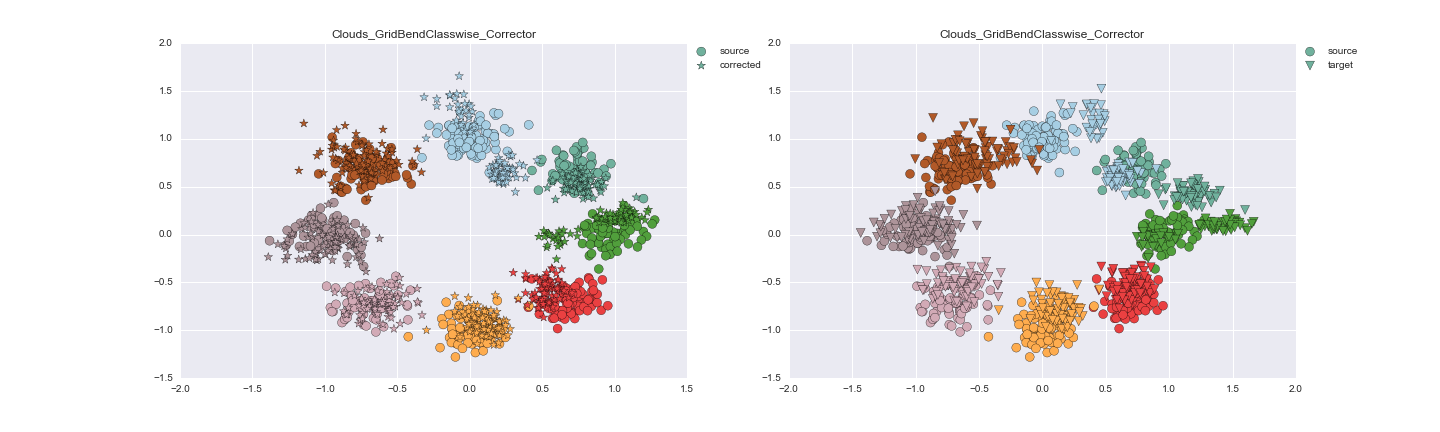
\includegraphics[width=\linewidth]{fig/24-05-2016/clouds/Clouds_GridBendClasswise_Corrector-DATA.png}
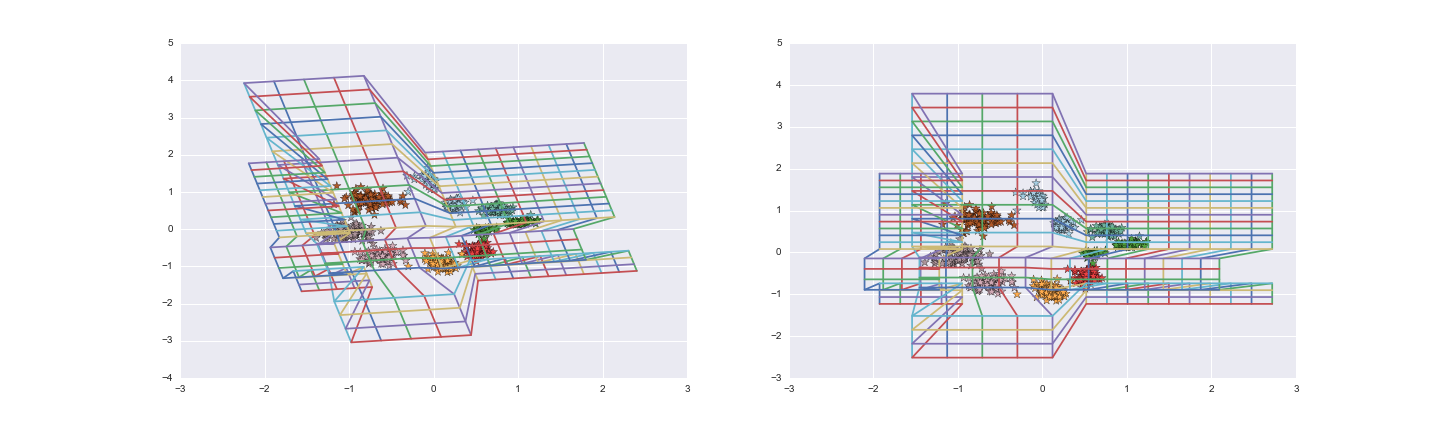
\includegraphics[width=\linewidth]{fig/24-05-2016/clouds/Clouds_GridBendClasswise_Corrector-GridCheck.png}
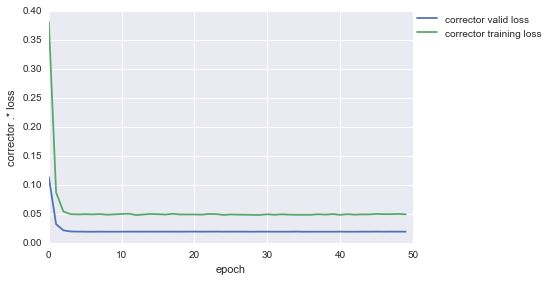
\includegraphics[width=0.45\linewidth]{fig/24-05-2016/clouds/Clouds_GridBendClasswise_Corrector-Learning_curve.png}
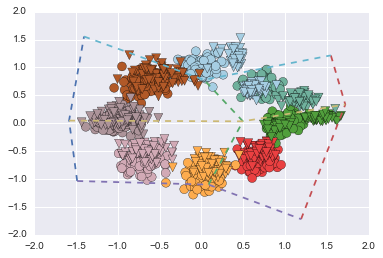
\includegraphics[width=0.45\linewidth]{fig/24-05-2016/clouds/cloud_grid.png}
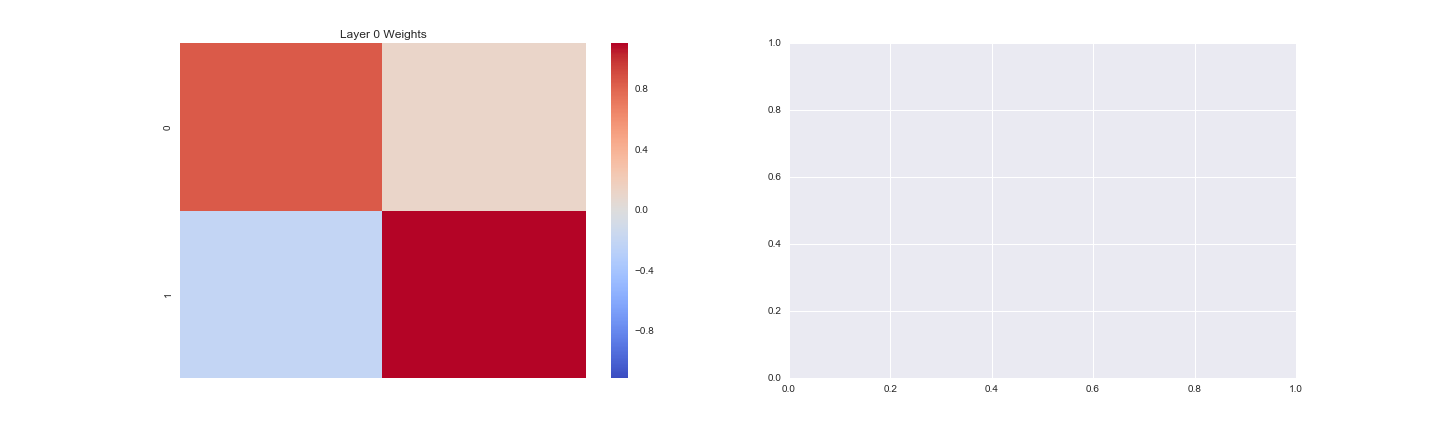
\includegraphics[width=\linewidth]{fig/24-05-2016/clouds/Clouds_GridBendClasswise_Corrector-W.png}
\caption{Correction de Clouds après application d'une transformation linéaire locale}
\label{fig:recap-clouds-GridBend-classwise}
\end{figure}


\subexperiment{Alignement appris : alignement au plus proche voisin au sein des classes}

{\Large \textbf{Rotation :}} On applique une rotation de 35 degrés par rapport à l'origine $(0,0)$.

\begin{figure}[H] % images
\centering
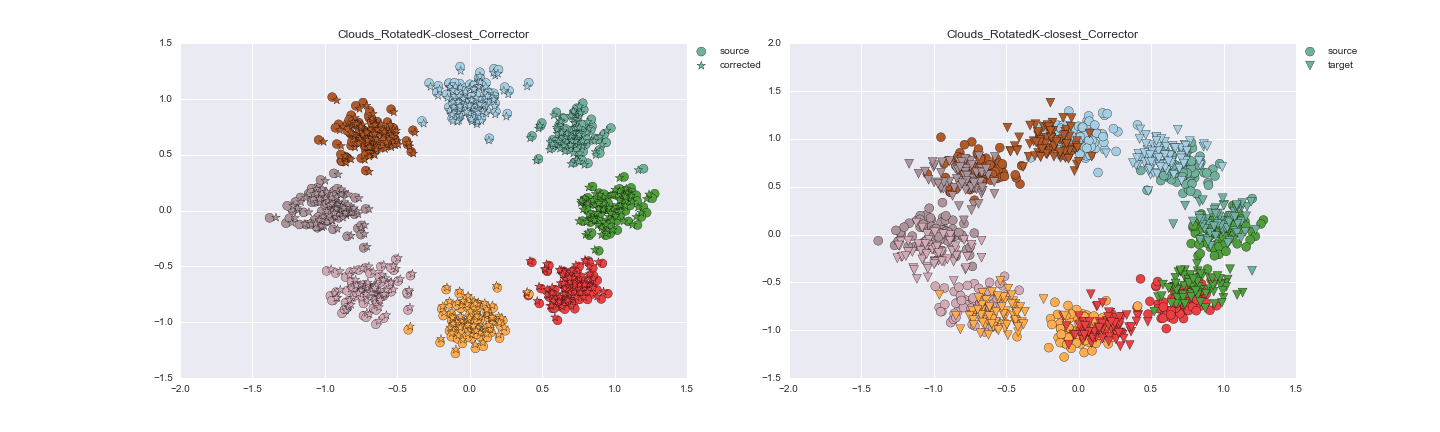
\includegraphics[width=\linewidth]{fig/24-05-2016/clouds/Clouds_RotatedK-closest_Corrector-DATA.png}
\includegraphics[width=\linewidth]{fig/24-05-2016/clouds/Clouds_RotatedK-closest_Corrector-GridCheck.png}
\includegraphics[width=0.45\linewidth]{fig/24-05-2016/clouds/Clouds_RotatedK-closest_Corrector-Learning_curve.png}
\includegraphics[width=\linewidth]{fig/24-05-2016/clouds/Clouds_RotatedK-closest_Corrector-W.png}
\caption{Correction de Clouds après une rotation de 35 degrés par rapport à l'origine avec les plus proches voisins entre les clusters}
\label{fig:recap-clouds-rot-exhaustive}
\end{figure}

{\Large \textbf{Random matrix :}}

\begin{figure}[H] % images
\centering
\includegraphics[width=\linewidth]{fig/24-05-2016/clouds/Clouds_RMatK-closest_Corrector-DATA.png}
\includegraphics[width=\linewidth]{fig/24-05-2016/clouds/Clouds_RMatK-closest_Corrector-GridCheck.png}
\includegraphics[width=0.45\linewidth]{fig/24-05-2016/clouds/Clouds_RMatK-closest_Corrector-Learning_curve.png}
\includegraphics[width=\linewidth]{fig/24-05-2016/clouds/Clouds_RMatK-closest_Corrector-W.png}
\caption{Correction de Clouds après multiplication par une matrice générée aléatoirement}
\label{fig:recap-clouds-RMat-exhaustive}
\end{figure}

{\Large \textbf{Grille tordue :}}

\begin{figure}[H] % images
\centering
\includegraphics[width=\linewidth]{fig/24-05-2016/clouds/Clouds_GridBendK-closest_Corrector-DATA.png}
\includegraphics[width=\linewidth]{fig/24-05-2016/clouds/Clouds_GridBendK-closest_Corrector-GridCheck.png}
\includegraphics[width=0.45\linewidth]{fig/24-05-2016/clouds/Clouds_GridBendK-closest_Corrector-Learning_curve.png}
\includegraphics[width=0.45\linewidth]{fig/24-05-2016/clouds/cloud_grid.png}
\includegraphics[width=\linewidth]{fig/24-05-2016/clouds/Clouds_GridBendK-closest_Corrector-W.png}
\caption{Correction de Clouds après application d'une transformation linéaire locale}
\label{fig:recap-clouds-GridBend-exhaustive}
\end{figure}

\subexperiment{Alignement appris : cluster plus proche}

{\Large \textbf{Rotation :}} On applique une rotation de 35 degrés par rapport à l'origine $(0,0)$.

\begin{figure}[H] % images
\centering
\includegraphics[width=\linewidth]{fig/24-05-2016/clouds/Clouds_RotatedCluster_Corrector-DATA.png}
\includegraphics[width=\linewidth]{fig/24-05-2016/clouds/Clouds_RotatedCluster_Corrector-GridCheck.png}
\includegraphics[width=0.45\linewidth]{fig/24-05-2016/clouds/Clouds_RotatedCluster_Corrector-Learning_curve.png}
\includegraphics[width=\linewidth]{fig/24-05-2016/clouds/Clouds_RotatedCluster_Corrector-W.png}
\caption{Correction de Clouds après une rotation de 35 degrés par rapport à l'origine avec les plus proches voisins entre les clusters}
\label{fig:recap-clouds-rot-cluster}
\end{figure}

{\Large \textbf{Random matrix :}}

\begin{figure}[H] % images
\centering
\includegraphics[width=\linewidth]{fig/24-05-2016/clouds/Clouds_RMatCluster_Corrector-DATA.png}
\includegraphics[width=\linewidth]{fig/24-05-2016/clouds/Clouds_RMatCluster_Corrector-GridCheck.png}
\includegraphics[width=0.45\linewidth]{fig/24-05-2016/clouds/Clouds_RMatCluster_Corrector-Learning_curve.png}
\includegraphics[width=\linewidth]{fig/24-05-2016/clouds/Clouds_RMatCluster_Corrector-W.png}
\caption{Correction de Clouds après multiplication par une matrice générée aléatoirement}
\label{fig:recap-clouds-RMat-cluster}
\end{figure}

{\Large \textbf{Grille tordue :}}

\begin{figure}[H] % images
\centering
\includegraphics[width=\linewidth]{fig/24-05-2016/clouds/Clouds_GridBendCluster_Corrector-DATA.png}
\includegraphics[width=\linewidth]{fig/24-05-2016/clouds/Clouds_GridBendCluster_Corrector-GridCheck.png}
\includegraphics[width=0.45\linewidth]{fig/24-05-2016/clouds/Clouds_GridBendCluster_Corrector-Learning_curve.png}
\includegraphics[width=0.45\linewidth]{fig/24-05-2016/clouds/cloud_grid.png}
\includegraphics[width=\linewidth]{fig/24-05-2016/clouds/Clouds_GridBendCluster_Corrector-W.png}
\caption{Correction de Clouds après application d'une transformation linéaire locale}
\label{fig:recap-clouds-GridBend-cluster}
\end{figure}


%%%%%%%%%%%%%%%%%%%%%%%%%%%%%%%%%%%%%%%%%%%%%%%%%%%%%%%%%%%%%%%%%%%%%%%%%%%%%%
%%%%%% CIRCLES
%%%%%%%%%%%%%%%%%%%%%%%%%%%%%%%%%%%%%%%%%%%%%%%%%%%%%%%%%%%%%%%%%%%%%%%%%%%%%%
\experiment{Circles}

\emph{Circles} est un jouet composé de $n$ classes ...

Toutes ces expériences ont été réaliséeses avec un learning rate de $0.1$ + un moment de $0.9$.


\subexperiment{Alignement connu}

Le cas où l'alignement est connu permet de vérifier que la transformation est facile ou non 
à inverser, les autres méthode ayant peu de chance de faire mieux.

{\Large \textbf{Rotation :}} On applique une rotation de 50 degrés par rapport à l'origine $(0,0)$.

\begin{figure}[H] % images
\centering
\includegraphics[width=\linewidth]{fig/24-05-2016/circles/Circles_RotatedPairwise_Corrector-DATA.png}
\includegraphics[width=\linewidth]{fig/24-05-2016/circles/Circles_RotatedPairwise_Corrector-GridCheck.png}
\includegraphics[width=0.45\linewidth]{fig/24-05-2016/circles/Circles_RotatedPairwise_Corrector-Learning_curve.png}
\includegraphics[width=\linewidth]{fig/24-05-2016/circles/Circles_RotatedPairwise_Corrector-W.png}
\caption{Correction de circles après une rotation de 50 degrés par rapport à l'origine avec alignement connu}
\label{fig:recap-circles-rot-pairwise}
\end{figure}

{\Large \textbf{Random matrix :}}

\begin{figure}[H] % images
\centering
\includegraphics[width=\linewidth]{fig/24-05-2016/circles/Circles_RMatPairwise_Corrector-DATA.png}
\includegraphics[width=\linewidth]{fig/24-05-2016/circles/Circles_RMatPairwise_Corrector-GridCheck.png}
\includegraphics[width=0.45\linewidth]{fig/24-05-2016/circles/Circles_RMatPairwise_Corrector-Learning_curve.png}
\includegraphics[width=\linewidth]{fig/24-05-2016/circles/Circles_RMatPairwise_Corrector-W.png}
\caption{Correction de circles après multiplication par une matrice générée aléatoirement}
\label{fig:recap-circles-RMat-pairwise}
\end{figure}


{\Large \textbf{Grille tordue :}}

\begin{figure}[H] % images
\centering
\includegraphics[width=\linewidth]{fig/24-05-2016/circles/Circles_GridBendPairwise_Corrector-DATA.png}
\includegraphics[width=\linewidth]{fig/24-05-2016/circles/Circles_GridBendPairwise_Corrector-GridCheck.png}
\includegraphics[width=0.45\linewidth]{fig/24-05-2016/circles/Circles_GridBendPairwise_Corrector-Learning_curve.png}
\includegraphics[width=0.45\linewidth]{fig/24-05-2016/circles/circles_grid.png}
\includegraphics[width=\linewidth]{fig/24-05-2016/circles/Circles_GridBendPairwise_Corrector-W.png}
\caption{Correction de circles après application d'une transformation linéaire locale}
\label{fig:recap-circles-GridBend-pairwise}
\end{figure}

\subexperiment{Alignement appris : alignement aléatoire au sein des classes}

{\Large \textbf{Rotation :}} On applique une rotation de 50 degrés par rapport à l'origine $(0,0)$.

\begin{figure}[H] % images
\centering
\includegraphics[width=\linewidth]{fig/24-05-2016/circles/Circles_RotatedClasswise_Corrector-DATA.png}
\includegraphics[width=\linewidth]{fig/24-05-2016/circles/Circles_RotatedClasswise_Corrector-GridCheck.png}
\includegraphics[width=0.45\linewidth]{fig/24-05-2016/circles/Circles_RotatedClasswise_Corrector-Learning_curve.png}
\includegraphics[width=\linewidth]{fig/24-05-2016/circles/Circles_RotatedClasswise_Corrector-W.png}
\caption{Correction de circles après une rotation de 50 degrés par rapport à l'origine avec les plus proches voisins entre les clusters}
\label{fig:recap-circles-rot-classwise}
\end{figure}

{\Large \textbf{Random matrix :}}

\begin{figure}[H] % images
\centering
\includegraphics[width=\linewidth]{fig/24-05-2016/circles/Circles_RMatClasswise_Corrector-DATA.png}
\includegraphics[width=\linewidth]{fig/24-05-2016/circles/Circles_RMatClasswise_Corrector-GridCheck.png}
\includegraphics[width=0.45\linewidth]{fig/24-05-2016/circles/Circles_RMatClasswise_Corrector-Learning_curve.png}
\includegraphics[width=\linewidth]{fig/24-05-2016/circles/Circles_RMatClasswise_Corrector-W.png}
\caption{Correction de circles après multiplication par une matrice générée aléatoirement}
\label{fig:recap-circles-RMat-classwise}
\end{figure}

{\Large \textbf{Grille tordue :}}

\begin{figure}[H] % images
\centering
\includegraphics[width=\linewidth]{fig/24-05-2016/circles/Circles_GridBendClasswise_Corrector-DATA.png}
\includegraphics[width=\linewidth]{fig/24-05-2016/circles/Circles_GridBendClasswise_Corrector-GridCheck.png}
\includegraphics[width=0.45\linewidth]{fig/24-05-2016/circles/Circles_GridBendClasswise_Corrector-Learning_curve.png}
\includegraphics[width=0.45\linewidth]{fig/24-05-2016/circles/circles_grid.png}
\includegraphics[width=\linewidth]{fig/24-05-2016/circles/Circles_GridBendClasswise_Corrector-W.png}
\caption{Correction de circles après application d'une transformation linéaire locale}
\label{fig:recap-circles-GridBend-classwise}
\end{figure}


\subexperiment{Alignement appris : alignement au plus proche voisin au sein des classes}

{\Large \textbf{Rotation :}} On applique une rotation de 50 degrés par rapport à l'origine $(0,0)$.

\begin{figure}[H] % images
\centering
\includegraphics[width=\linewidth]{fig/24-05-2016/circles/Circles_RotatedK-closest_Corrector-DATA.png}
\includegraphics[width=\linewidth]{fig/24-05-2016/circles/Circles_RotatedK-closest_Corrector-GridCheck.png}
\includegraphics[width=0.45\linewidth]{fig/24-05-2016/circles/Circles_RotatedK-closest_Corrector-Learning_curve.png}
\includegraphics[width=\linewidth]{fig/24-05-2016/circles/Circles_RotatedK-closest_Corrector-W.png}
\caption{Correction de circles après une rotation de 50 degrés par rapport à l'origine avec les plus proches voisins entre les clusters}
\label{fig:recap-circles-rot-exhaustive}
\end{figure}

{\Large \textbf{Random matrix :}}

\begin{figure}[H] % images
\centering
\includegraphics[width=\linewidth]{fig/24-05-2016/circles/Circles_RMatK-closest_Corrector-DATA.png}
\includegraphics[width=\linewidth]{fig/24-05-2016/circles/Circles_RMatK-closest_Corrector-GridCheck.png}
\includegraphics[width=0.45\linewidth]{fig/24-05-2016/circles/Circles_RMatK-closest_Corrector-Learning_curve.png}
\includegraphics[width=\linewidth]{fig/24-05-2016/circles/Circles_RMatK-closest_Corrector-W.png}
\caption{Correction de circles après multiplication par une matrice générée aléatoirement}
\label{fig:recap-circles-RMat-exhaustive}
\end{figure}

{\Large \textbf{Grille tordue :}}

\begin{figure}[H] % images
\centering
\includegraphics[width=\linewidth]{fig/24-05-2016/circles/Circles_GridBendK-closest_Corrector-DATA.png}
\includegraphics[width=\linewidth]{fig/24-05-2016/circles/Circles_GridBendK-closest_Corrector-GridCheck.png}
\includegraphics[width=0.45\linewidth]{fig/24-05-2016/circles/Circles_GridBendK-closest_Corrector-Learning_curve.png}
\includegraphics[width=0.45\linewidth]{fig/24-05-2016/circles/circles_grid.png}
\includegraphics[width=\linewidth]{fig/24-05-2016/circles/Circles_GridBendK-closest_Corrector-W.png}
\caption{Correction de circles après application d'une transformation linéaire locale}
\label{fig:recap-circles-GridBend-exhaustive}
\end{figure}

\subexperiment{Alignement appris : cluster plus proche}

{\Large \textbf{Rotation :}} On applique une rotation de 50 degrés par rapport à l'origine $(0,0)$.

\begin{figure}[H] % images
\centering
\includegraphics[width=\linewidth]{fig/24-05-2016/circles/Circles_RotatedCluster_Corrector-DATA.png}
\includegraphics[width=\linewidth]{fig/24-05-2016/circles/Circles_RotatedCluster_Corrector-GridCheck.png}
\includegraphics[width=0.45\linewidth]{fig/24-05-2016/circles/Circles_RotatedCluster_Corrector-Learning_curve.png}
\includegraphics[width=\linewidth]{fig/24-05-2016/circles/Circles_RotatedCluster_Corrector-W.png}
\caption{Correction de circles après une rotation de 50 degrés par rapport à l'origine avec les plus proches voisins entre les clusters}
\label{fig:recap-circles-rot-cluster}
\end{figure}

{\Large \textbf{Random matrix :}}

\begin{figure}[H] % images
\centering
\includegraphics[width=\linewidth]{fig/24-05-2016/circles/Circles_RMatCluster_Corrector-DATA.png}
\includegraphics[width=\linewidth]{fig/24-05-2016/circles/Circles_RMatCluster_Corrector-GridCheck.png}
\includegraphics[width=0.45\linewidth]{fig/24-05-2016/circles/Circles_RMatCluster_Corrector-Learning_curve.png}
\includegraphics[width=\linewidth]{fig/24-05-2016/circles/Circles_RMatCluster_Corrector-W.png}
\caption{Correction de circles après multiplication par une matrice générée aléatoirement}
\label{fig:recap-circles-RMat-cluster}
\end{figure}

{\Large \textbf{Grille tordue :}}

\begin{figure}[H] % images
\centering
\includegraphics[width=\linewidth]{fig/24-05-2016/circles/Circles_GridBendCluster_Corrector-DATA.png}
\includegraphics[width=\linewidth]{fig/24-05-2016/circles/Circles_GridBendCluster_Corrector-GridCheck.png}
\includegraphics[width=0.45\linewidth]{fig/24-05-2016/circles/Circles_GridBendCluster_Corrector-Learning_curve.png}
\includegraphics[width=0.45\linewidth]{fig/24-05-2016/circles/circles_grid.png}
\includegraphics[width=\linewidth]{fig/24-05-2016/circles/Circles_GridBendCluster_Corrector-W.png}
\caption{Correction de circles après application d'une transformation linéaire locale}
\label{fig:recap-circles-GridBend-cluster}
\end{figure}

%%%%%%%%%%%%%%%%%%%%%%%%%%%%%%%%%%%%%%%%%%%%%%%%%%%%%%%%%%%%%%%%%%%%%%%%%%%%%%
%%%%%% X
%%%%%%%%%%%%%%%%%%%%%%%%%%%%%%%%%%%%%%%%%%%%%%%%%%%%%%%%%%%%%%%%%%%%%%%%%%%%%%

\experiment{X}

\emph{X} est un jouet composé de $n$ classes 

Toutes ces expériences ont été réalisées avec un learning rate de $0.1$ + un moment de $0.9$.


\subexperiment{Alignement connu}
Le cas où l'alignement est connu permet de vérifier que la transformation est facile ou non 
à inverser, les autres méthode ayant peu de chance de faire mieux.

{\Large \textbf{Rotation :}} On applique une rotation de 50 degrés par rapport à l'origine $(0,0)$.

\begin{figure}[H] % images
\centering
\includegraphics[width=\linewidth]{fig/24-05-2016/X/X_RotatedPairwise_Corrector-DATA.png}
\includegraphics[width=\linewidth]{fig/24-05-2016/X/X_RotatedPairwise_Corrector-GridCheck.png}
\includegraphics[width=0.45\linewidth]{fig/24-05-2016/X/X_RotatedPairwise_Corrector-Learning_curve.png}
\includegraphics[width=\linewidth]{fig/24-05-2016/X/X_RotatedPairwise_Corrector-W.png}
\caption{Correction de X après une rotation de 50 degrés par rapport à l'origine avec alignement connu}
\label{fig:recap-X-rot-pairwise}
\end{figure}

{\Large \textbf{Random matrix :}}

\begin{figure}[H] % images
\centering
\includegraphics[width=\linewidth]{fig/24-05-2016/X/X_RMatPairwise_Corrector-DATA.png}
\includegraphics[width=\linewidth]{fig/24-05-2016/X/X_RMatPairwise_Corrector-GridCheck.png}
\includegraphics[width=0.45\linewidth]{fig/24-05-2016/X/X_RMatPairwise_Corrector-Learning_curve.png}
\includegraphics[width=\linewidth]{fig/24-05-2016/X/X_RMatPairwise_Corrector-W.png}
\caption{Correction de X après multiplication par une matrice générée aléatoirement}
\label{fig:recap-X-RMat-pairwise}
\end{figure}


{\Large \textbf{Grille tordue :}}

\begin{figure}[H] % images
\centering
\includegraphics[width=\linewidth]{fig/24-05-2016/X/X_GridBendPairwise_Corrector-DATA.png}
\includegraphics[width=\linewidth]{fig/24-05-2016/X/X_GridBendPairwise_Corrector-GridCheck.png}
\includegraphics[width=0.45\linewidth]{fig/24-05-2016/X/X_GridBendPairwise_Corrector-Learning_curve.png}
\includegraphics[width=0.45\linewidth]{fig/24-05-2016/X/X_grid.png}
\includegraphics[width=\linewidth]{fig/24-05-2016/X/X_GridBendPairwise_Corrector-W.png}
\caption{Correction de X après application d'une transformation linéaire locale}
\label{fig:recap-X-GridBend-pairwise}
\end{figure}

\subexperiment{Alignement appris : alignement aléatoire au sein des classes}

{\Large \textbf{Rotation :}} On applique une rotation de 50 degrés par rapport à l'origine $(0,0)$.

\begin{figure}[H] % images
\centering
\includegraphics[width=\linewidth]{fig/24-05-2016/X/X_RotatedClasswise_Corrector-DATA.png}
\includegraphics[width=\linewidth]{fig/24-05-2016/X/X_RotatedClasswise_Corrector-GridCheck.png}
\includegraphics[width=0.45\linewidth]{fig/24-05-2016/X/X_RotatedClasswise_Corrector-Learning_curve.png}
\includegraphics[width=\linewidth]{fig/24-05-2016/X/X_RotatedClasswise_Corrector-W.png}
\caption{Correction de X après une rotation de 50 degrés par rapport à l'origine avec les plus proches voisins entre les clusters}
\label{fig:recap-X-rot-classwise}
\end{figure}

{\Large \textbf{Random matrix :}}

\begin{figure}[H] % images
\centering
\includegraphics[width=\linewidth]{fig/24-05-2016/X/X_RMatClasswise_Corrector-DATA.png}
\includegraphics[width=\linewidth]{fig/24-05-2016/X/X_RMatClasswise_Corrector-GridCheck.png}
\includegraphics[width=0.45\linewidth]{fig/24-05-2016/X/X_RMatClasswise_Corrector-Learning_curve.png}
\includegraphics[width=\linewidth]{fig/24-05-2016/X/X_RMatClasswise_Corrector-W.png}
\caption{Correction de X après multiplication par une matrice générée aléatoirement}
\label{fig:recap-X-RMat-classwise}
\end{figure}

{\Large \textbf{Grille tordue :}}

\begin{figure}[H] % images
\centering
\includegraphics[width=\linewidth]{fig/24-05-2016/X/X_GridBendClasswise_Corrector-DATA.png}
\includegraphics[width=\linewidth]{fig/24-05-2016/X/X_GridBendClasswise_Corrector-GridCheck.png}
\includegraphics[width=0.45\linewidth]{fig/24-05-2016/X/X_GridBendClasswise_Corrector-Learning_curve.png}
\includegraphics[width=0.45\linewidth]{fig/24-05-2016/X/X_grid.png}
\includegraphics[width=\linewidth]{fig/24-05-2016/X/X_GridBendClasswise_Corrector-W.png}
\caption{Correction de X après application d'une transformation linéaire locale}
\label{fig:recap-X-GridBend-classwise}
\end{figure}


\subexperiment{Alignement appris : alignement au plus proche voisin au sein des classes}

{\Large \textbf{Rotation :}} On applique une rotation de 50 degrés par rapport à l'origine $(0,0)$.

\begin{figure}[H] % images
\centering
\includegraphics[width=\linewidth]{fig/24-05-2016/X/X_RotatedK-closest_Corrector-DATA.png}
\includegraphics[width=\linewidth]{fig/24-05-2016/X/X_RotatedK-closest_Corrector-GridCheck.png}
\includegraphics[width=0.45\linewidth]{fig/24-05-2016/X/X_RotatedK-closest_Corrector-Learning_curve.png}
\includegraphics[width=\linewidth]{fig/24-05-2016/X/X_RotatedK-closest_Corrector-W.png}
\caption{Correction de X après une rotation de 50 degrés par rapport à l'origine avec les plus proches voisins entre les clusters}
\label{fig:recap-X-rot-exhaustive}
\end{figure}

{\Large \textbf{Random matrix :}}

\begin{figure}[H] % images
\centering
\includegraphics[width=\linewidth]{fig/24-05-2016/X/X_RMatK-closest_Corrector-DATA.png}
\includegraphics[width=\linewidth]{fig/24-05-2016/X/X_RMatK-closest_Corrector-GridCheck.png}
\includegraphics[width=0.45\linewidth]{fig/24-05-2016/X/X_RMatK-closest_Corrector-Learning_curve.png}
\includegraphics[width=\linewidth]{fig/24-05-2016/X/X_RMatK-closest_Corrector-W.png}
\caption{Correction de X après multiplication par une matrice générée aléatoirement}
\label{fig:recap-X-RMat-exhaustive}
\end{figure}

{\Large \textbf{Grille tordue :}}

\begin{figure}[H] % images
\centering
\includegraphics[width=\linewidth]{fig/24-05-2016/X/X_GridBendK-closest_Corrector-DATA.png}
\includegraphics[width=\linewidth]{fig/24-05-2016/X/X_GridBendK-closest_Corrector-GridCheck.png}
\includegraphics[width=0.45\linewidth]{fig/24-05-2016/X/X_GridBendK-closest_Corrector-Learning_curve.png}
\includegraphics[width=0.45\linewidth]{fig/24-05-2016/X/X_grid.png}
\includegraphics[width=\linewidth]{fig/24-05-2016/X/X_GridBendK-closest_Corrector-W.png}
\caption{Correction de X après application d'une transformation linéaire locale}
\label{fig:recap-X-GridBend-exhaustive}
\end{figure}

\subexperiment{Alignement appris : cluster plus proche}

{\Large \textbf{Rotation :}} On applique une rotation de 50 degrés par rapport à l'origine $(0,0)$.

\begin{figure}[H] % images
\centering
\includegraphics[width=\linewidth]{fig/24-05-2016/X/X_RotatedCluster_Corrector-DATA.png}
\includegraphics[width=\linewidth]{fig/24-05-2016/X/X_RotatedCluster_Corrector-GridCheck.png}
\includegraphics[width=0.45\linewidth]{fig/24-05-2016/X/X_RotatedCluster_Corrector-Learning_curve.png}
\includegraphics[width=\linewidth]{fig/24-05-2016/X/X_RotatedCluster_Corrector-W.png}
\caption{Correction de X après une rotation de 50 degrés par rapport à l'origine avec les plus proches voisins entre les clusters}
\label{fig:recap-X-rot-cluster}
\end{figure}

{\Large \textbf{Random matrix :}}

\begin{figure}[H] % images
\centering
\includegraphics[width=\linewidth]{fig/24-05-2016/X/X_RMatCluster_Corrector-DATA.png}
\includegraphics[width=\linewidth]{fig/24-05-2016/X/X_RMatCluster_Corrector-GridCheck.png}
\includegraphics[width=0.45\linewidth]{fig/24-05-2016/X/X_RMatCluster_Corrector-Learning_curve.png}
\includegraphics[width=\linewidth]{fig/24-05-2016/X/X_RMatCluster_Corrector-W.png}
\caption{Correction de X après multiplication par une matrice générée aléatoirement}
\label{fig:recap-X-RMat-cluster}
\end{figure}

{\Large \textbf{Grille tordue :}}

\begin{figure}[H] % images
\centering
\includegraphics[width=\linewidth]{fig/24-05-2016/X/X_GridBendCluster_Corrector-DATA.png}
\includegraphics[width=\linewidth]{fig/24-05-2016/X/X_GridBendCluster_Corrector-GridCheck.png}
\includegraphics[width=0.45\linewidth]{fig/24-05-2016/X/X_GridBendCluster_Corrector-Learning_curve.png}
\includegraphics[width=0.45\linewidth]{fig/24-05-2016/X/X_grid.png}
\includegraphics[width=\linewidth]{fig/24-05-2016/X/X_GridBendCluster_Corrector-W.png}
\caption{Correction de X après application d'une transformation linéaire locale}
\label{fig:recap-X-GridBend-cluster}
\end{figure}

%%%%%%%%%%%%%%%%%%%%%%%%%%%%%%%%%%%%%%%%%%%%%%%%%%%%%%%%%%%%%%%%%%%%%%%%%%%%%%
%%%%%% MOONS
%%%%%%%%%%%%%%%%%%%%%%%%%%%%%%%%%%%%%%%%%%%%%%%%%%%%%%%%%%%%%%%%%%%%%%%%%%%%%%

\experiment{Moons}

\emph{Moons} est un jouet composé de $n$ classes (nuages de point gaussiens) se partageant 
l'espace sur le cercle unité.

Toutes ces expériences ont été réalisées avec un learning rate de $0.1$ + un moment de $0.9$.


\subexperiment{Alignement connu}
Le cas où l'alignement est connu permet de vérifier que la transformation est facile ou non 
à inverser, les autres méthode ayant peu de chance de faire mieux.

{\Large \textbf{Rotation :}} On applique une rotation de 50 degrés par rapport à l'origine $(0,0)$.

\begin{figure}[H] % images
\centering
\includegraphics[width=\linewidth]{fig/24-05-2016/moons/Moons_RotatedPairwise_Corrector-DATA.png}
\includegraphics[width=\linewidth]{fig/24-05-2016/moons/Moons_RotatedPairwise_Corrector-GridCheck.png}
\includegraphics[width=0.45\linewidth]{fig/24-05-2016/moons/Moons_RotatedPairwise_Corrector-Learning_curve.png}
\includegraphics[width=\linewidth]{fig/24-05-2016/moons/Moons_RotatedPairwise_Corrector-W.png}
\caption{Correction de moons après une rotation de 50 degrés par rapport à l'origine avec alignement connu}
\label{fig:recap-moons-rot-pairwise}
\end{figure}

{\Large \textbf{Random matrix :}}

\begin{figure}[H] % images
\centering
\includegraphics[width=\linewidth]{fig/24-05-2016/moons/Moons_RMatPairwise_Corrector-DATA.png}
\includegraphics[width=\linewidth]{fig/24-05-2016/moons/Moons_RMatPairwise_Corrector-GridCheck.png}
\includegraphics[width=0.45\linewidth]{fig/24-05-2016/moons/Moons_RMatPairwise_Corrector-Learning_curve.png}
\includegraphics[width=\linewidth]{fig/24-05-2016/moons/Moons_RMatPairwise_Corrector-W.png}
\caption{Correction de moons après multiplication par une matrice générée aléatoirement}
\label{fig:recap-moons-RMat-pairwise}
\end{figure}


{\Large \textbf{Grille tordue :}}

\begin{figure}[H] % images
\centering
\includegraphics[width=\linewidth]{fig/24-05-2016/moons/Moons_GridBendPairwise_Corrector-DATA.png}
\includegraphics[width=\linewidth]{fig/24-05-2016/moons/Moons_GridBendPairwise_Corrector-GridCheck.png}
\includegraphics[width=0.45\linewidth]{fig/24-05-2016/moons/Moons_GridBendPairwise_Corrector-Learning_curve.png}
\includegraphics[width=0.45\linewidth]{fig/24-05-2016/moons/moons_grid.png}
\includegraphics[width=\linewidth]{fig/24-05-2016/moons/Moons_GridBendPairwise_Corrector-W.png}
\caption{Correction de moons après application d'une transformation linéaire locale}
\label{fig:recap-moons-GridBend-pairwise}
\end{figure}

\subexperiment{Alignement appris : alignement aléatoire au sein des classes}

{\Large \textbf{Rotation :}} On applique une rotation de 50 degrés par rapport à l'origine $(0,0)$.

\begin{figure}[H] % images
\centering
\includegraphics[width=\linewidth]{fig/24-05-2016/moons/Moons_RotatedClasswise_Corrector-DATA.png}
\includegraphics[width=\linewidth]{fig/24-05-2016/moons/Moons_RotatedClasswise_Corrector-GridCheck.png}
\includegraphics[width=0.45\linewidth]{fig/24-05-2016/moons/Moons_RotatedClasswise_Corrector-Learning_curve.png}
\includegraphics[width=\linewidth]{fig/24-05-2016/moons/Moons_RotatedClasswise_Corrector-W.png}
\caption{Correction de moons après une rotation de 50 degrés par rapport à l'origine avec les plus proches voisins entre les clusters}
\label{fig:recap-moons-rot-classwise}
\end{figure}

{\Large \textbf{Random matrix :}}

\begin{figure}[H] % images
\centering
\includegraphics[width=\linewidth]{fig/24-05-2016/moons/Moons_RMatClasswise_Corrector-DATA.png}
\includegraphics[width=\linewidth]{fig/24-05-2016/moons/Moons_RMatClasswise_Corrector-GridCheck.png}
\includegraphics[width=0.45\linewidth]{fig/24-05-2016/moons/Moons_RMatClasswise_Corrector-Learning_curve.png}
\includegraphics[width=\linewidth]{fig/24-05-2016/moons/Moons_RMatClasswise_Corrector-W.png}
\caption{Correction de moons après multiplication par une matrice générée aléatoirement}
\label{fig:recap-moons-RMat-classwise}
\end{figure}

{\Large \textbf{Grille tordue :}}

\begin{figure}[H] % images
\centering
\includegraphics[width=\linewidth]{fig/24-05-2016/moons/Moons_GridBendClasswise_Corrector-DATA.png}
\includegraphics[width=\linewidth]{fig/24-05-2016/moons/Moons_GridBendClasswise_Corrector-GridCheck.png}
\includegraphics[width=0.45\linewidth]{fig/24-05-2016/moons/Moons_GridBendClasswise_Corrector-Learning_curve.png}
\includegraphics[width=0.45\linewidth]{fig/24-05-2016/moons/moons_grid.png}
\includegraphics[width=\linewidth]{fig/24-05-2016/moons/Moons_GridBendClasswise_Corrector-W.png}
\caption{Correction de moons après application d'une transformation linéaire locale}
\label{fig:recap-moons-GridBend-classwise}
\end{figure}


\subexperiment{Alignement appris : alignement au plus proche voisin au sein des classes}

{\Large \textbf{Rotation :}} On applique une rotation de 50 degrés par rapport à l'origine $(0,0)$.

\begin{figure}[H] % images
\centering
\includegraphics[width=\linewidth]{fig/24-05-2016/moons/Moons_RotatedK-closest_Corrector-DATA.png}
\includegraphics[width=\linewidth]{fig/24-05-2016/moons/Moons_RotatedK-closest_Corrector-GridCheck.png}
\includegraphics[width=0.45\linewidth]{fig/24-05-2016/moons/Moons_RotatedK-closest_Corrector-Learning_curve.png}
\includegraphics[width=\linewidth]{fig/24-05-2016/moons/Moons_RotatedK-closest_Corrector-W.png}
\caption{Correction de moons après une rotation de 50 degrés par rapport à l'origine avec les plus proches voisins entre les clusters}
\label{fig:recap-moons-rot-exhaustive}
\end{figure}

{\Large \textbf{Random matrix :}}

\begin{figure}[H] % images
\centering
\includegraphics[width=\linewidth]{fig/24-05-2016/moons/Moons_RMatK-closest_Corrector-DATA.png}
\includegraphics[width=\linewidth]{fig/24-05-2016/moons/Moons_RMatK-closest_Corrector-GridCheck.png}
\includegraphics[width=0.45\linewidth]{fig/24-05-2016/moons/Moons_RMatK-closest_Corrector-Learning_curve.png}
\includegraphics[width=\linewidth]{fig/24-05-2016/moons/Moons_RMatK-closest_Corrector-W.png}
\caption{Correction de moons après multiplication par une matrice générée aléatoirement}
\label{fig:recap-moons-RMat-exhaustive}
\end{figure}

{\Large \textbf{Grille tordue :}}

\begin{figure}[H] % images
\centering
\includegraphics[width=\linewidth]{fig/24-05-2016/moons/Moons_GridBendK-closest_Corrector-DATA.png}
\includegraphics[width=\linewidth]{fig/24-05-2016/moons/Moons_GridBendK-closest_Corrector-GridCheck.png}
\includegraphics[width=0.45\linewidth]{fig/24-05-2016/moons/Moons_GridBendK-closest_Corrector-Learning_curve.png}
\includegraphics[width=0.45\linewidth]{fig/24-05-2016/moons/moons_grid.png}
\includegraphics[width=\linewidth]{fig/24-05-2016/moons/Moons_GridBendK-closest_Corrector-W.png}
\caption{Correction de moons après application d'une transformation linéaire locale}
\label{fig:recap-moons-GridBend-exhaustive}
\end{figure}

\subexperiment{Alignement appris : cluster plus proche}

{\Large \textbf{Rotation :}} On applique une rotation de 50 degrés par rapport à l'origine $(0,0)$.

\begin{figure}[H] % images
\centering
\includegraphics[width=\linewidth]{fig/24-05-2016/moons/Moons_RotatedCluster_Corrector-DATA.png}
\includegraphics[width=\linewidth]{fig/24-05-2016/moons/Moons_RotatedCluster_Corrector-GridCheck.png}
\includegraphics[width=0.45\linewidth]{fig/24-05-2016/moons/Moons_RotatedCluster_Corrector-Learning_curve.png}
\includegraphics[width=\linewidth]{fig/24-05-2016/moons/Moons_RotatedCluster_Corrector-W.png}
\caption{Correction de moons après une rotation de 50 degrés par rapport à l'origine avec les plus proches voisins entre les clusters}
\label{fig:recap-moons-rot-cluster}
\end{figure}

{\Large \textbf{Random matrix :}}

\begin{figure}[H] % images
\centering
\includegraphics[width=\linewidth]{fig/24-05-2016/moons/Moons_RMatCluster_Corrector-DATA.png}
\includegraphics[width=\linewidth]{fig/24-05-2016/moons/Moons_RMatCluster_Corrector-GridCheck.png}
\includegraphics[width=0.45\linewidth]{fig/24-05-2016/moons/Moons_RMatCluster_Corrector-Learning_curve.png}
\includegraphics[width=\linewidth]{fig/24-05-2016/moons/Moons_RMatCluster_Corrector-W.png}
\caption{Correction de moons après multiplication par une matrice générée aléatoirement}
\label{fig:recap-moons-RMat-cluster}
\end{figure}

{\Large \textbf{Grille tordue :}}

\begin{figure}[H] % images
\centering
\includegraphics[width=\linewidth]{fig/24-05-2016/moons/Moons_GridBendCluster_Corrector-DATA.png}
\includegraphics[width=\linewidth]{fig/24-05-2016/moons/Moons_GridBendCluster_Corrector-GridCheck.png}
\includegraphics[width=0.45\linewidth]{fig/24-05-2016/moons/Moons_GridBendCluster_Corrector-Learning_curve.png}
\includegraphics[width=0.45\linewidth]{fig/24-05-2016/moons/moons_grid.png}
\includegraphics[width=\linewidth]{fig/24-05-2016/moons/Moons_GridBendCluster_Corrector-W.png}
\caption{Correction de moons après application d'une transformation linéaire locale}
\label{fig:recap-moons-GridBend-cluster}
\end{figure}


%----------------------------------------------------------------------------------------



%----------------------------------------------------------------------------------------
%	FORMULAE AND MEDIA RECIPES
%----------------------------------------------------------------------------------------

% \labday{} % We don't want a date here so we make the labday blank

% Big title !
% \begin{center}
% \HRule \\[0.4cm]
% {\huge \textbf{Jolie titre !}}\\[0.4cm] % Heading
% \HRule \\[1.5cm]
% \end{center}

%----------------------------------------------------------------------------------------
%	FORMULAE
%----------------------------------------------------------------------------------------

% \newpage

% \huge \textbf{Formulae} \\ \\

% \normalsize \textbf{Formula 1 - Pythagorean theorem}\\ \\
% $a^2 + b^2 = c^2$\\ \\

%-----------------------------------------

%\textbf{Formula X - Description}\\ \\

%Formula

%----------------------------------------------------------------------------------------

\end{document}